%%%%%%%%%%%%%%%%%%%%%%%%%%%%%%%%%%%%%%%%%%%%%%%%%%%%%%%%%%%%%%%%%%%%%%%%%%%%%%%%
%2345678901234567890123456789012345678901234567890123456789012345678901234567890
%        1         2         3         4         5         6         7         8

%\documentclass[letterpaper, 10 pt, conference]{ieeeconf}  % Comment this line out
                                                          % if you need a4paper
\documentclass[a4paper, 10pt, conference]{ieeeconf}      % Use this line for a4
                                                          % paper

\IEEEoverridecommandlockouts                              % This command is only
                                                          % needed if you want to
                                                          % use the \thanks command
\overrideIEEEmargins
% See the \addtolength command later in the file to balance the column lengths
% on the last page of the document

\usepackage{graphicx}
\usepackage[margin=1in]{geometry}
\usepackage{hyperref}
\usepackage{amsmath}
\usepackage{mathrsfs}
\usepackage{float}

\DeclareMathOperator{\card}{card}
\DeclareMathOperator{\trc}{tr}
\DeclareMathOperator{\mean}{mean}
\DeclareMathOperator{\bin}{bin}
\DeclareMathOperator{\lns}{lanes}
\DeclareMathOperator{\cnt}{count}

\bibliographystyle{ieeetr}

% The following packages can be found on http:\\www.ctan.org
%\usepackage{graphics} % for pdf, bitmapped graphics files
%\usepackage{epsfig} % for postscript graphics files
%\usepackage{mathptmx} % assumes new font selection scheme installed
%\usepackage{times} % assumes new font selection scheme installed
%\usepackage{amsmath} % assumes amsmath package installed
%\usepackage{amssymb}  % assumes amsmath package installed

\title{\LARGE \bf
Linearized Aw-Rascle-Zhang Model for Road Traffic Prediction and Control
}

%\author{ \parbox{3 in}{\centering Huibert Kwakernaak*
%         \thanks{*Use the $\backslash$thanks command to put information here}\\
%         Faculty of Electrical Engineering, Mathematics and Computer Science\\
%         University of Twente\\
%         7500 AE Enschede, The Netherlands\\
%         {\tt\small h.kwakernaak@autsubmit.com}}
%         \hspace*{ 0.5 in}
%         \parbox{3 in}{ \centering Pradeep Misra**
%         \thanks{**The footnote marks may be inserted manually}\\
%        Department of Electrical Engineering \\
%         Wright State University\\
%         Dayton, OH 45435, USA\\
%         {\tt\small pmisra@cs.wright.edu}}
%}

\author{Francois Belletti, Mandy Huo, Xavier Litrico, Alexandre M. Bayen}

\begin{document}

\maketitle
\thispagestyle{empty}
\pagestyle{empty}

\begin{abstract}
This article starts from the classical Aw-Rascle-Zhang (ARZ) model for freeway traffic and develops a spectral analysis of its linearized version. A counterpart to the Froude number in hydrodynamics is defined that enables a classification of the nature of vehicle traffic flow using the explicit solution resulting from the analysis. We prove that our linearization about an equilibrium is stable for congested regimes and unstable otherwise. NGSIM data for congested traffic trajectories is used so as to confront the linearized model's predictions to actual macroscopic behavior of traffic. The model is shown to achieve good accuracy for speed and flow. In particular, it replicates the propagation of boundary conditions' oscillations into the interior resolution domain of the PDE under study.
\end{abstract}

%\linenumbers

\section{Introduction}

Researchers aiming at devising control strategies for road traffic face a trade-off between empirical evidence confirming the accuracy of non-linear models \cite{zielke2008empirical, Jamitons2008} and the easiness of use of linear systems when it comes to designing controllers.

Non-linear second order models such as Payne-Whitham \cite{payne1971models, whitham1974linear} were first presented as a compelling alternative to first order models \cite{LW, Richards} that accounted for many features observed empirically in traffic such as stop-and-go behavior. Although Daganzo highlighted many flaws of the first generation of that family of models \cite{Dag_requiem}, a second generation including the Aw-Rascle equations \cite{AR} and phase transition models \cite{colombo2003hyperbolic} offered a step towards more realism in macroscopic traffic modeling.

The Aw-Rascle-Zhang model -- one of the most accurate in that group -- accounts for persisting oscillations, information propagation anisotropy and drivers' impulse to shorten their travel times. Linearizing the ARZ model, based on the analogous work of Litrico \cite{litrico2009modeling} for Saint-Venant equations, offers a unique opportunity to work in a realistic modeling framework where the phenomena mentioned above are accounted for and, at the same time, use linear control theory and spectral Laplace analysis.

Our approach in this paper is therefore to linearize the ARZ model about an equilibrium so as to make the best of a trade-off between model accuracy and easiness of use. The first section is dedicated to the linearization and spectral analysis of the ARZ model. We prove there is convective instability in free-flow regime that drives the model away from its equilibrium  state and devise an equivalent of the hydrodynamics' Froud number for traffic macroscopic models. Laplace transforms and low frequency analysis also enable a tractable interpretation of the underlying dynamics of the system. The second section focuses on the accuracy of the resulting linear equations. It confronts their predictions with ground truth data extracted from the NGSIM data set for the US-101 freeway.

\section{The ARZ model} \label{ARZSection}

We consider the ARZ model with relaxation term. The model is shown here:
{\footnotesize
\begin{align} 
\footnotesize
\rho_t + (\rho v)_x &= 0, \label{ARZ1} \\
(v - V(\rho))_t + v(v - V(\rho))_x &=\dfrac{V(\rho) - v}{\tau} \label{ARZ2},
\end{align}
}
where $\rho$ is the density, $v$ is the velocity, $\tau$ is the relaxation time, and {\footnotesize$V(\rho) = Q(\rho)/\rho$} is the equilibrium velocity profile. Finally $Q(\rho)$ is the density-flow relation given by the fundamental diagram. We assume that $V$ is $C^{1}$ derivable over its domain.

In vector form the ARZ model is
{\footnotesize
\begin{equation} \label{ARZrhov}
\begin{pmatrix}
	\rho \\
	v
\end{pmatrix}_t
+ 
\begin{pmatrix}
	v & \rho \\
	0 & v + \rho V' (\rho)
\end{pmatrix}
\begin{pmatrix}
	\rho \\ 
	v
\end{pmatrix}_x = 
\begin{pmatrix}
	0 \\ 
	\dfrac{V(\rho) - v}{\tau}
\end{pmatrix}
\end{equation}
}

With the appropriate change of variable, we can rewrite the model in the density-flow and velocity-flow forms, the latter of which is most useful to us for practical control purposes. Using the flow relation $q = \rho v$ and \eqref{ARZrhov}, the speed-flow form is

{\footnotesize
\begin{subequations}
\begin{align}
\footnotesize
\begin{pmatrix}
	v \\ 
	q
\end{pmatrix}_t
+ C\left(v, q\right)&
\begin{pmatrix}
	v \\ 
	q
\end{pmatrix}_x 
=
\dfrac{1}{\tau}
\begin{pmatrix}
	V\left( \frac{q}{v}\right) - v \\
	Q\left( \frac{q}{v}\right) - q
\end{pmatrix}. \label{ARZvq} \\
C\left(v, q \right)
&=
\begin{pmatrix}
	v + \frac{q}{v} V'\left( \frac{q}{v} \right) & 0 \\
	\frac{q}{v} \left( v + \frac{q}{v} V'\left( \frac{q}{v} \right) \right) & v
\end{pmatrix}
\end{align}
\end{subequations}
}

The $\left(v, q \right)$ form has seldom been used in transportation engineering however it is promising for data fusion purposes that involve both loop detector measurements (providing values for $q$) and GPS traces (giving estimates for $v$).


\subsection{Linearization}
We are interested in small deviations, {\footnotesize$(\tilde{\rho}(x,t), \tilde{v}(x,t))$}, from a given nominal profile. Consider the nominal solution {\footnotesize$(\rho^*(x),v^*(x))(V(\rho^*) = v^*)$} satisfying {\footnotesize$v_t = \rho_t = 0$}. Then \eqref{ARZrhov} becomes
{\footnotesize
\begin{align}
v^* \rho^*_x + v^*_x\rho^* = 0, \\
( v^* + \rho^* V'( \rho^*) )v^*_x = \dfrac{V(\rho^*) - v^*}{\tau} = 0.
\end{align}
}
Then we must have {\footnotesize$v^*_x=\rho^*_x=0$}, so the solution is uniform along the road. 

we linearize about the equilibrium {\footnotesize$(\rho^*, q^*)(\rho^*V(\rho^*) = q^*)$} with deviations {\footnotesize$(\tilde{\rho}(x,t), \tilde{q}(x,t))$}.

This last form presented below \eqref{linARZvq} is most adapted to traffic prediction and control in practical settings where flows and vehicle velocities are measured. The following will focus on deriving an explicit solution to these equations.

{\footnotesize
\begin{subequations} \label{linARZvq}
\begin{align}
&\begin{pmatrix}
	\tilde{\rho} \\
	\tilde{v}
\end{pmatrix}_t
+ \bar{C}
\begin{pmatrix}
	\tilde{\rho} \\ 
	\tilde{v}
\end{pmatrix}_x 
= 
\bar{B}
\begin{pmatrix}
	\tilde{\rho} \\
	\tilde{v}
\end{pmatrix}, \\
&\bar{C} 
=
\begin{pmatrix}
	v^* + \frac{q^*}{v^*} V'\left(\frac{q^*}{v^*}\right) & 0 \\
	\frac{q^*}{v^*} \left( v^* + \frac{q^*}{v^*} V'\left(\frac{q^*}{v^*}\right)\right) & v^*
\end{pmatrix} \\
&\bar{B} 
=
\frac{1}{v^{*}\tau}
\begin{pmatrix}
		-\dfrac{(v^*)^2+q^*V'\left(\frac{q^*}{v^*}\right)}{v^*} & V'\left(\frac{q^*}{v^*}\right) \\
		-\dfrac{q^*\left((v^*)^2 + q^*V'\left(\frac{q^*}{v^*}\right)\right)}{(v^*)^2}  & \dfrac{q^*V'\left(\frac{q^*}{v^*}\right)}{v^*}
\end{pmatrix}
\end{align}
\end{subequations}
}


\subsection{Characteristic form}

Diagonalization of the velocity-flow yields
{\footnotesize
\begin{equation} \label{vqlindiag}
\begin{pmatrix}
\xi_1 \\ \xi_2
\end{pmatrix}_t + 
\underset{A}{
	\underbrace{
	\begin{pmatrix}
		\lambda_1 & 0 \\
		0 & \lambda_2
	\end{pmatrix} 
	}
}
\begin{pmatrix}
\xi_1 \\ \xi_2
\end{pmatrix}_x = 
\underset{B}{
	\underbrace{
	\begin{pmatrix}
		-\frac{1}{\tau} & 0 \\
		-\frac{1}{\tau} & 0
	\end{pmatrix}}
}
\begin{pmatrix}
\xi_1 \\ \xi_2
\end{pmatrix},
\end{equation}
}
where the eigen values, {\footnotesize$\lambda_1 = v^{*}$ and $\lambda_2 = v^{*} + \frac{q^{*}}{v^{*}} V'(\frac{q^{*}}{v^{*}})$, $\xi_1 = \dfrac{\rho^*\lambda_2}{\lambda_1 - \lambda_2}\tilde{v} + \tilde{q}$} and {\footnotesize$\xi_2 = \dfrac{q^*}{\lambda_1 - \lambda_2}\tilde{v}$}.
Therefore this is consistent with the physical dynamics of the system as no waves travel faster than the equilibrium vehicle speed.\\

\subsection{The Traffic Froude Number}
In fluid mechanics, the Froude number is a dimensionless number which delineates the boundary between flow regimes \cite{Sturm, litrico2009modeling}. Using the eigenvalues of the system in the characteristic form, we are able to define a useful counterpart to this number. 
Since {\footnotesize $V(\rho)$} is non-increasing function, we have {\footnotesize $V'(\rho^*) \leq 0$}. Assuming {\footnotesize$V'(\rho^*) \neq 0$} there are two flow regimes: one in which {\footnotesize$\lambda_1 \lambda_2 < 0$} and one characteristic line travels downstream whereas the other characteristic line travels upstream, and one in which {\footnotesize$\lambda_1 \lambda_2 > 0$} and both characteristic lines travel downstream. We define the \textit{Traffic Froude Number} (TFN) as
{\footnotesize
\begin{equation}
F = \left\lvert\dfrac{\rho^*V'( \rho^*)}{v^*}\right\rvert.
\end{equation}
}
Then we have
{\footnotesize
\begin{equation*}
\begin{cases}
F > 1 &\Rightarrow |\rho^*V'(\rho^*)| > v^* \quad \Rightarrow \lambda_2  <0 \\
F < 1 &\Rightarrow |\rho^*V'(\rho^*)| < v^* \quad \Rightarrow \lambda_2 > 0
\end{cases}.
\end{equation*}
}
Hence the system is in free-flow when $F<1$ and congestion when $F>1$. In hydrodynamics these regimes are referred to as the subcritical and supercritical regimes, respectively \cite{litrico2009modeling}. The direction of characteristic lines is illustrated in Figure \ref{Characteristics}. Note also that {\footnotesize$\lambda_2 = v^* + \rho^* V'( \rho^*) = \dfrac{Q(\rho^*)}{\rho^*} + \dfrac{\rho^*Q'(\rho^*)-Q(\rho^*)}{\rho^*} = Q'(\rho^*)$}.

For traffic, the interpretation of the different regimes is somewhat different. Free flow regime corresponds to these situations where drivers are not slowed down by heavy traffic and go as fast as the desired speed. The congested regime arises when traffic is denser and, because too many cars are present on the same freeway section, drivers slow down and eventually form traffic jam.

\begin{figure}
\begin{centering}
\begin{tabular}{cc}
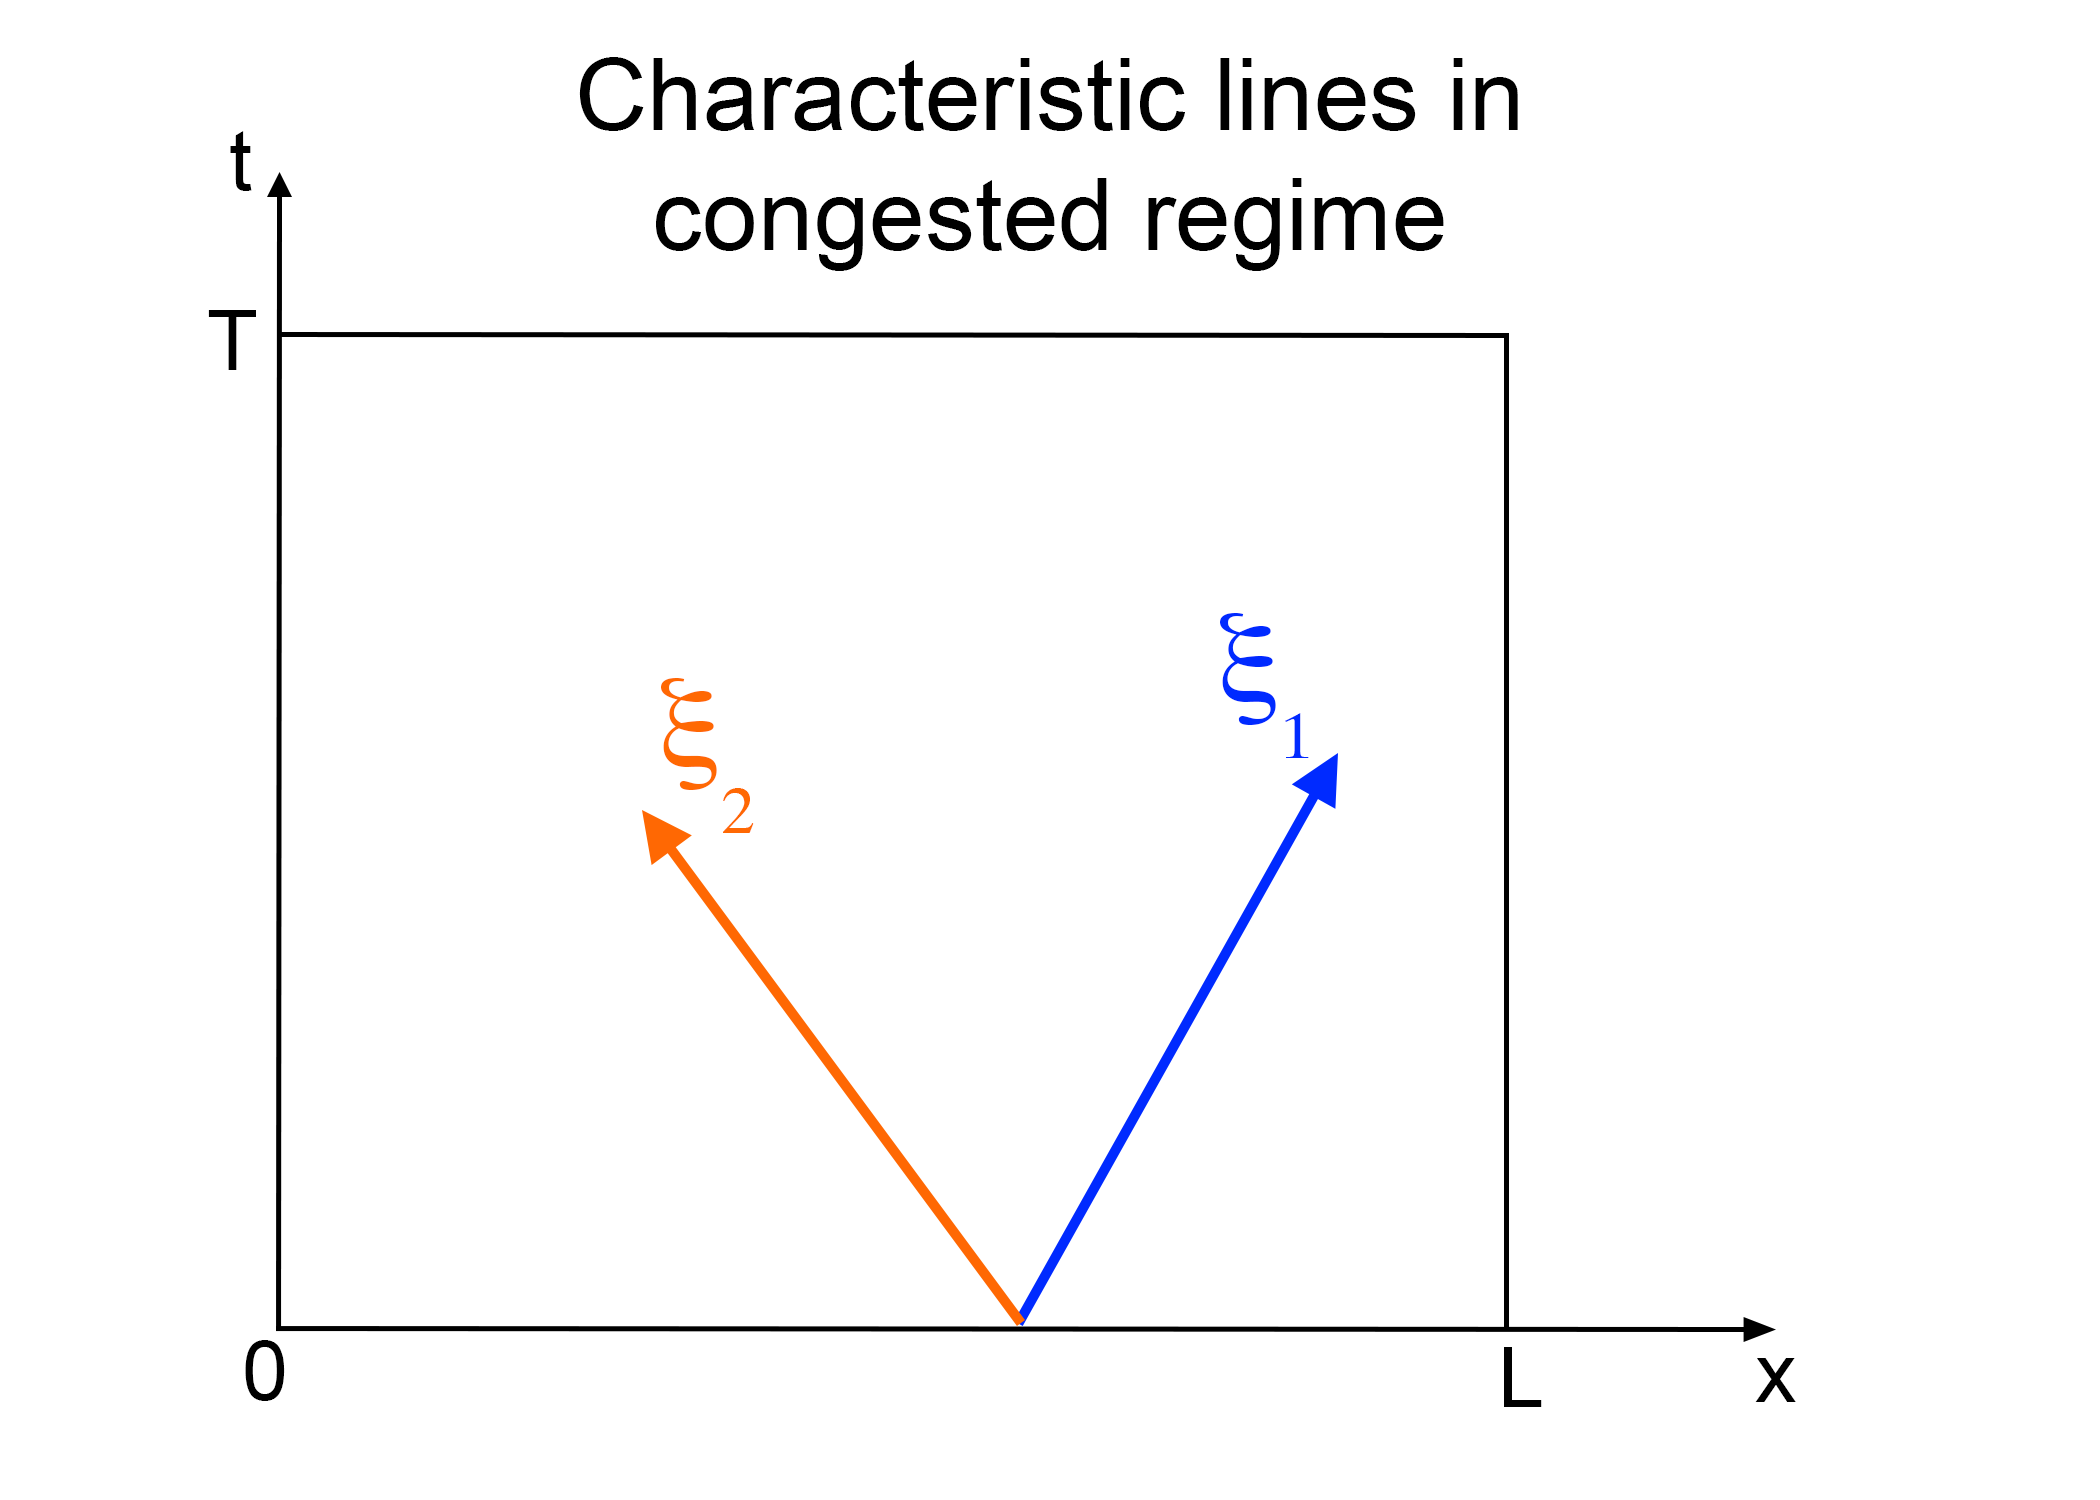
\includegraphics[width=4cm]{Congested-regime} & 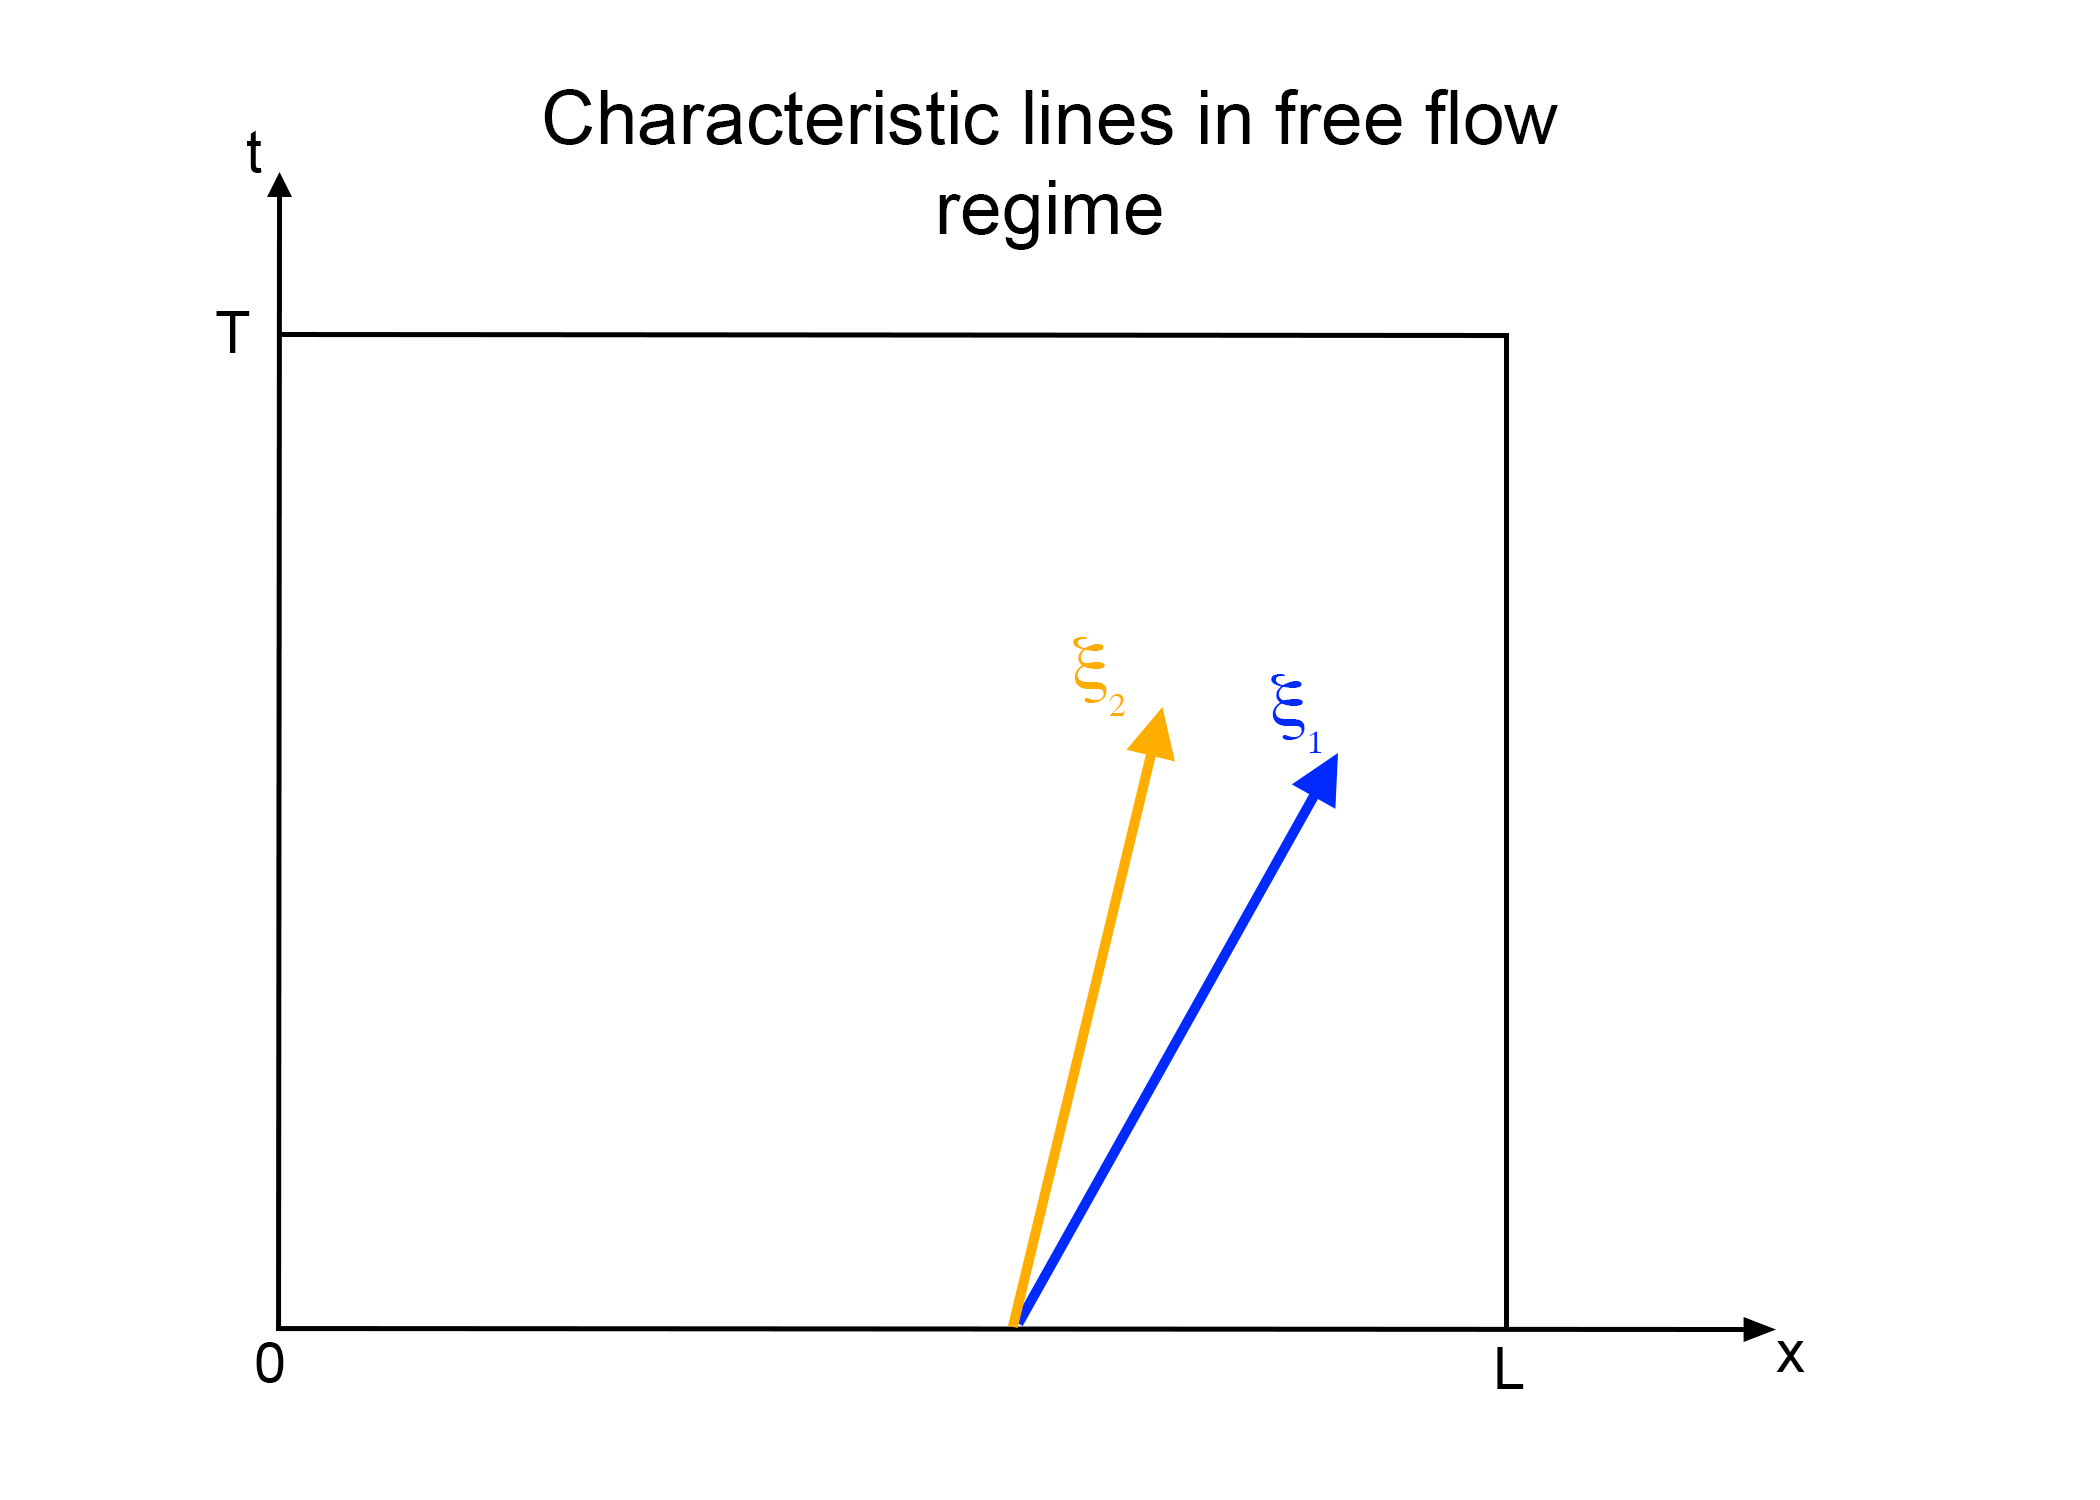
\includegraphics[width=4cm]{Free-flow-regime}\tabularnewline
$F>1$, $\lambda_{2}<0$, $\lambda_{1}>0$ & $F<1$, $\lambda_{1}>\lambda_{2}>0$\tabularnewline
\end{tabular}
\par\end{centering}
\protect\caption{Illustration of characteristic lines in congested (supercritical) and free-flow regime (subcritical) $\xi_1$ and $\xi_2$ propagate along.\label{Characteristics}}
\end{figure}


\section{Spectral analysis of the linearized ARZ model}
We now consider the $(v,q)$ system for the frequency domain analysis for practical control purposes.

\subsection{State-transition matrix}
Taking the Laplace transform of the diagonalized form \eqref{vqlindiag} we obtain 
{\footnotesize
$\dfrac{\partial \hat{\xi} (x,s)}{\partial x} = \mathscr{A}(s)\hat{\xi}(x,s) + \mathscr{B}\xi(x,t=0^-)$
}
where {\footnotesize$\mathscr{A}(s) = A^{-1}(\tilde{B} - sI)$} and {\footnotesize $\mathscr{B} = -A^{-1}$}. Assuming zero initial conditions we have 
{\footnotesize \label{TFRiemann}
$\hat{\xi}(x,s) = \Phi(x,s)\hat{\xi}(0,s)$
}
where {\footnotesize$\Phi(x,s) = e^{\mathscr{A}(s)x}$} is the state-transition matrix.

To compute the exponential we diagonalize the matrix $\mathscr{A}(s)$
which then yields the components of $\Phi(x,s)$:
{\footnotesize
\begin{subequations} \label{TFv0q0tovxqx}
\begin{align}
\phi_{11}(x,s) &= e^{-\frac{x}{\tau \lambda_1}}e^{-\frac{x}{\lambda_1}s}, \\ 
\phi_{12}(x,s) &= 0, \\
\phi_{21}(x,s) &= \dfrac{\lambda_1 \left( e^{-\frac{x}{\tau \lambda_1}}e^{-\frac{x}{\lambda_1}s} - e^{-\frac{x}{\lambda_2}s}\right)}{\lambda_2 - \tau (\lambda_1 - \lambda_2)s}, \\
\phi_{22}(x,s) &= e^{-\frac{x}{\lambda_2}s}.
\end{align}
\end{subequations}
}

\subsection{Free-flow case ($F<1$)}
Consider the system in the free-flow regime. With $\xi_1 (0,t)$ and $\xi_2 (0,t)$ as the inputs and $\xi_1(L,t)$ and $\xi_2(L,t)$ as the outputs, the distributed transfer matrix is exactly the state-transition matrix $\Phi(x,s)$. Inverting the linear transform that gives $\xi_1$ and $\xi_2$ as functions of $v$ and $q$, we can write
{\footnotesize
$\label{vqfreeflow}
\begin{pmatrix}
	\widetilde{v}(x,s) \\ 
	\widetilde{q}(x,s)
\end{pmatrix} = 
\Psi(x,s)
\begin{pmatrix}
	\widetilde{v}(0,s) \\ 
	\widetilde{q}(0,s)
\end{pmatrix}
$
}
where, letting {\footnotesize$\alpha = -\dfrac{\lambda_2}{\tau(\lambda_1 - \lambda_2)}$},
{\footnotesize
\begin{subequations}
\begin{align}
\psi_{11}(x,s) &= 
\frac{
	\alpha e^{-\frac{x}{\lambda_{1}}\left(s+\frac{1}{\tau}\right)}
		+ s e^{-\frac{sx}{\lambda_{2}}}
}{
	s + \alpha
}, \\
\psi_{12}(x,s) &=
\frac{1}{\rho^* \tau}
\frac{
	e^{-\frac{sx}{\lambda_{2}}}
	-
	e^{-\frac{x}{\lambda_{1}}\left(s+\frac{1}		{\tau}\right)}
}{
	s + \alpha
}, \\
\psi_{21}(x,s) &=
- s \rho^{*} \tau \alpha
\frac{
	e^{-\frac{sx}{\lambda_{2}}}
	-
	e^{-\frac{x}{\lambda_{1}}\left(s+\frac{1}		{\tau}\right)}
}{
	s + \alpha
}, \\
\psi_{22}(x,s) &=
\frac{
	s e^{-\frac{x}{\lambda_{1}}\left(s+\frac{1}{\tau}\right)}
		+ \alpha e^{-\frac{sx}{\lambda_{2}}}
}{
	s + \alpha
}.
\end{align}
\end{subequations}
}

We have $\frac{1}{\lambda_{1}}\left(-\alpha+\frac{1}{\tau}\right) = \frac{-\alpha}{\lambda_{2}}$, thus a Taylor expansion about $-\alpha$ shows that numerators and denominators cancel each other out for $s \rightarrow -\alpha$. This proves that the output remains bounded for a given value of $x$. We will show below that a conic region of the $\left[0,T\right] \times \left[0,L\right]$ domain features exponential growth in free-flow regime. This arises when changing $t$ and $x$ simultaneously and complements the conclusion formulated above.\\

\subsubsection{Low frequency approximation for physical variables in free-flow regime}
Analyzing the expressions above becomes easier when approximating them for $\left|s\right|\ll\left|\alpha\right|$. This corresponds to traffic flow varying slowly and smoothly. We find the following approximate expressions for the transfer functions:
{\footnotesize
\begin{subequations}
\begin{align}
\psi_{11}(x,s)
&\simeq
e^{-\frac{sx}{\lambda_{2}}}
e^{-\frac{x}{\tau\lambda_{1}}}
, \\
\psi_{12}(x,s)
&\simeq
\frac{
	1
}{
	\rho^{*}\tau\alpha
}
e^{-\frac{sx}{\lambda_{2}}}
\left(
	1 - e^{-\frac{x}{\tau\lambda_{1}}}
\right)
, \\
\psi_{21}(x,s)
& \simeq
- s \rho^{*} \tau
e^{-\frac{sx}{\lambda_{2}}}
\left(
	1 - e^{-\frac{x}{\tau\lambda_{1}}}
\right)
, \\
\psi_{22}(x,s)
&\simeq
e^{-\frac{sx}{\lambda_{2}}}
.
\end{align}
\end{subequations}
}

Interpreting the low frequency expressions is fairly straightforward in terms of distributed delays featuring $\lambda_1$ or $\lambda_2$ as information propagation speeds and distributed gains where $\lambda_1 \tau$ is the characteristic damping distance. It is also remarkable that $\widetilde{q}(x,s)$ appears as the result of a derivator applied to $\widetilde{v}(0,s)$.\\

\subsubsection{Bode plots for free-flow regime}

We generate Bode plots using the following parameters taken from \cite{Hofleitner}: $q_{\text{max}}$ = 1300 veh/h, $\rho_{\text{max}}$ = 0.1 veh/m, and $L$ = 100 m. The Greenshields fundamental diagram, {\footnotesize $Q( \rho) = 4 \frac{q_{\text{max}}}{\rho_{\text{max}}^2}\rho (\rho_{\text{max}} - \rho)$}, is used to approximate the fundamental diagram. For inhomogeneous second-order models, the relaxation time, $\tau$, falls in the range of about 14-60 seconds \cite{Fan}. A relaxation time of $\tau$ = 15 s is used for the following simulations. We simulate for $\rho^* = 0.01$ veh/m. Here the characteristic frequency of the system, $\left|\alpha\right|$, equals 0.53 Hz which is indeed sensible for traffic flow modeling.

The Bode plots for the physical variables are displayed in Figure \ref{fig:Magn_spatial_physx}.

\begin{figure}
\centering
\begin{tabular}{cc}
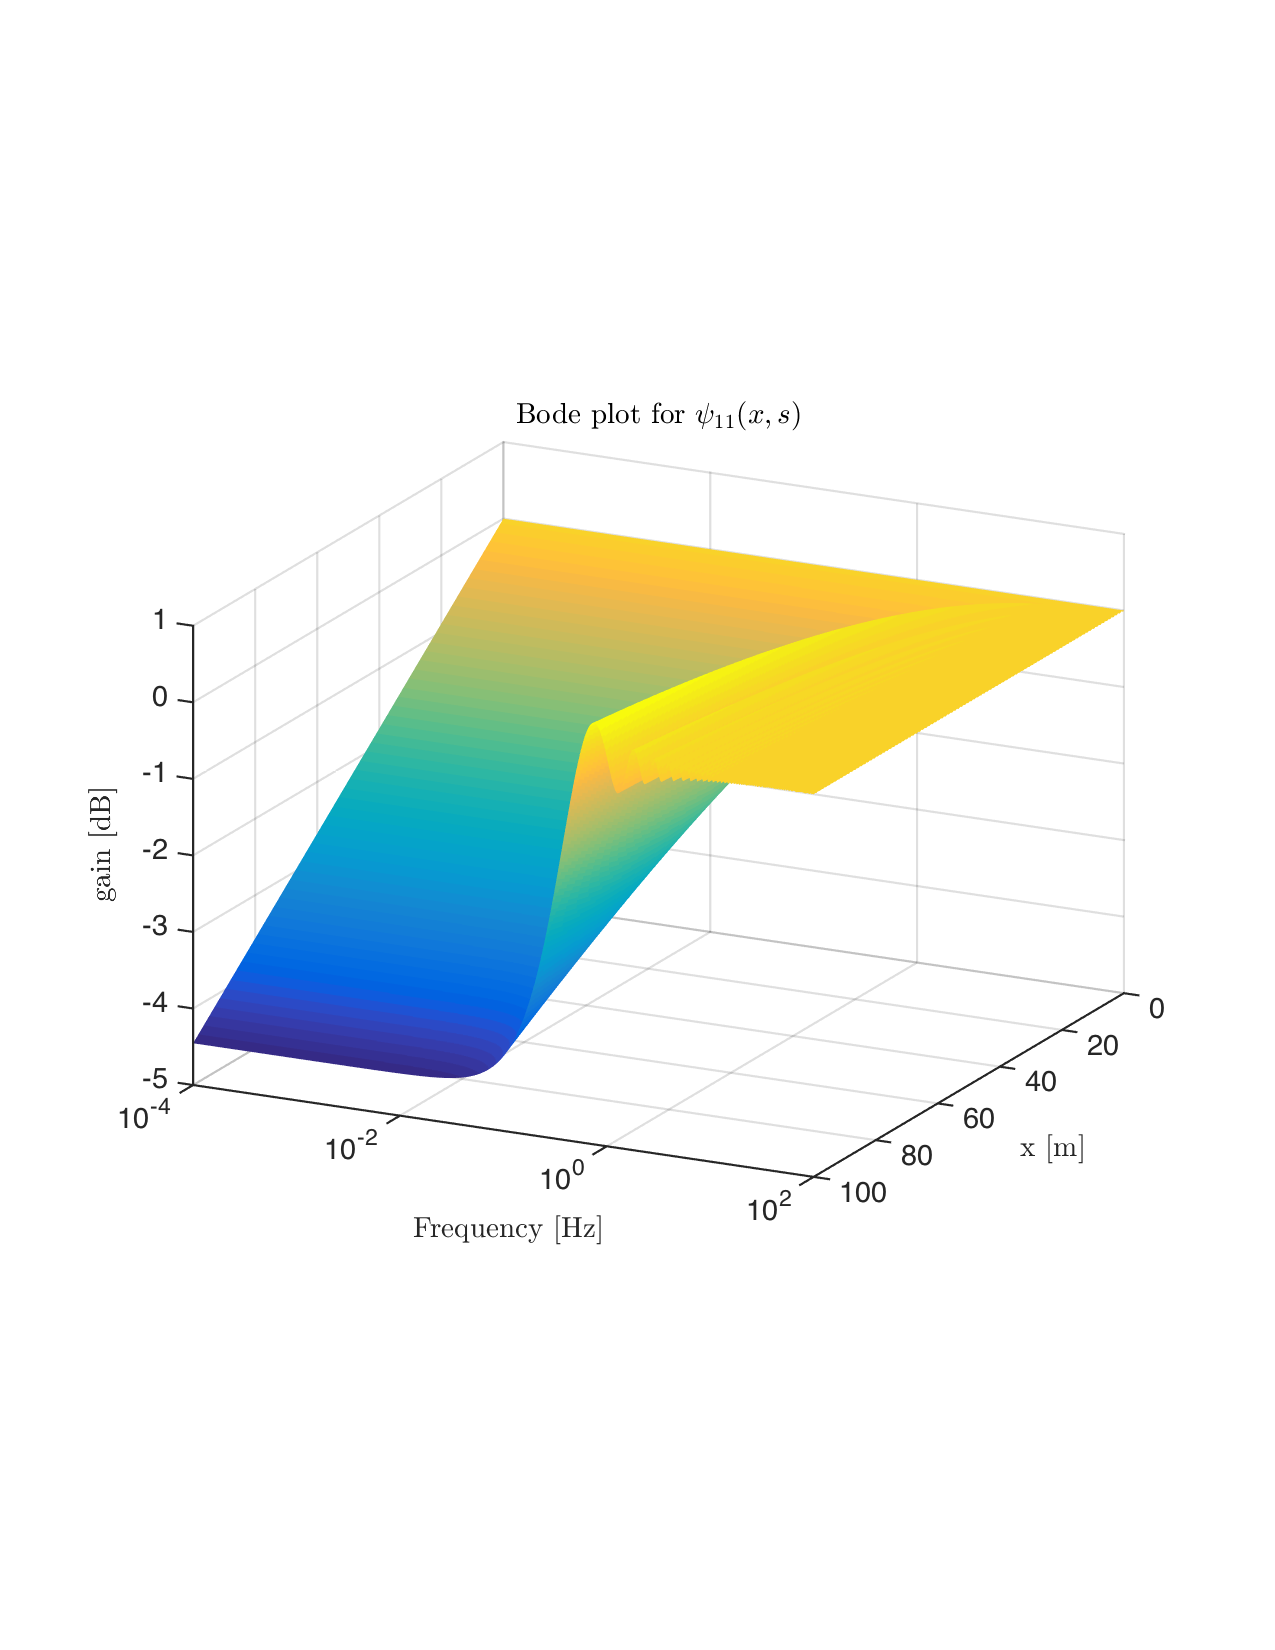
\includegraphics[trim = 0mm 60mm 0mm 60mm, width = 3.9cm]{distr_psi_11}
&
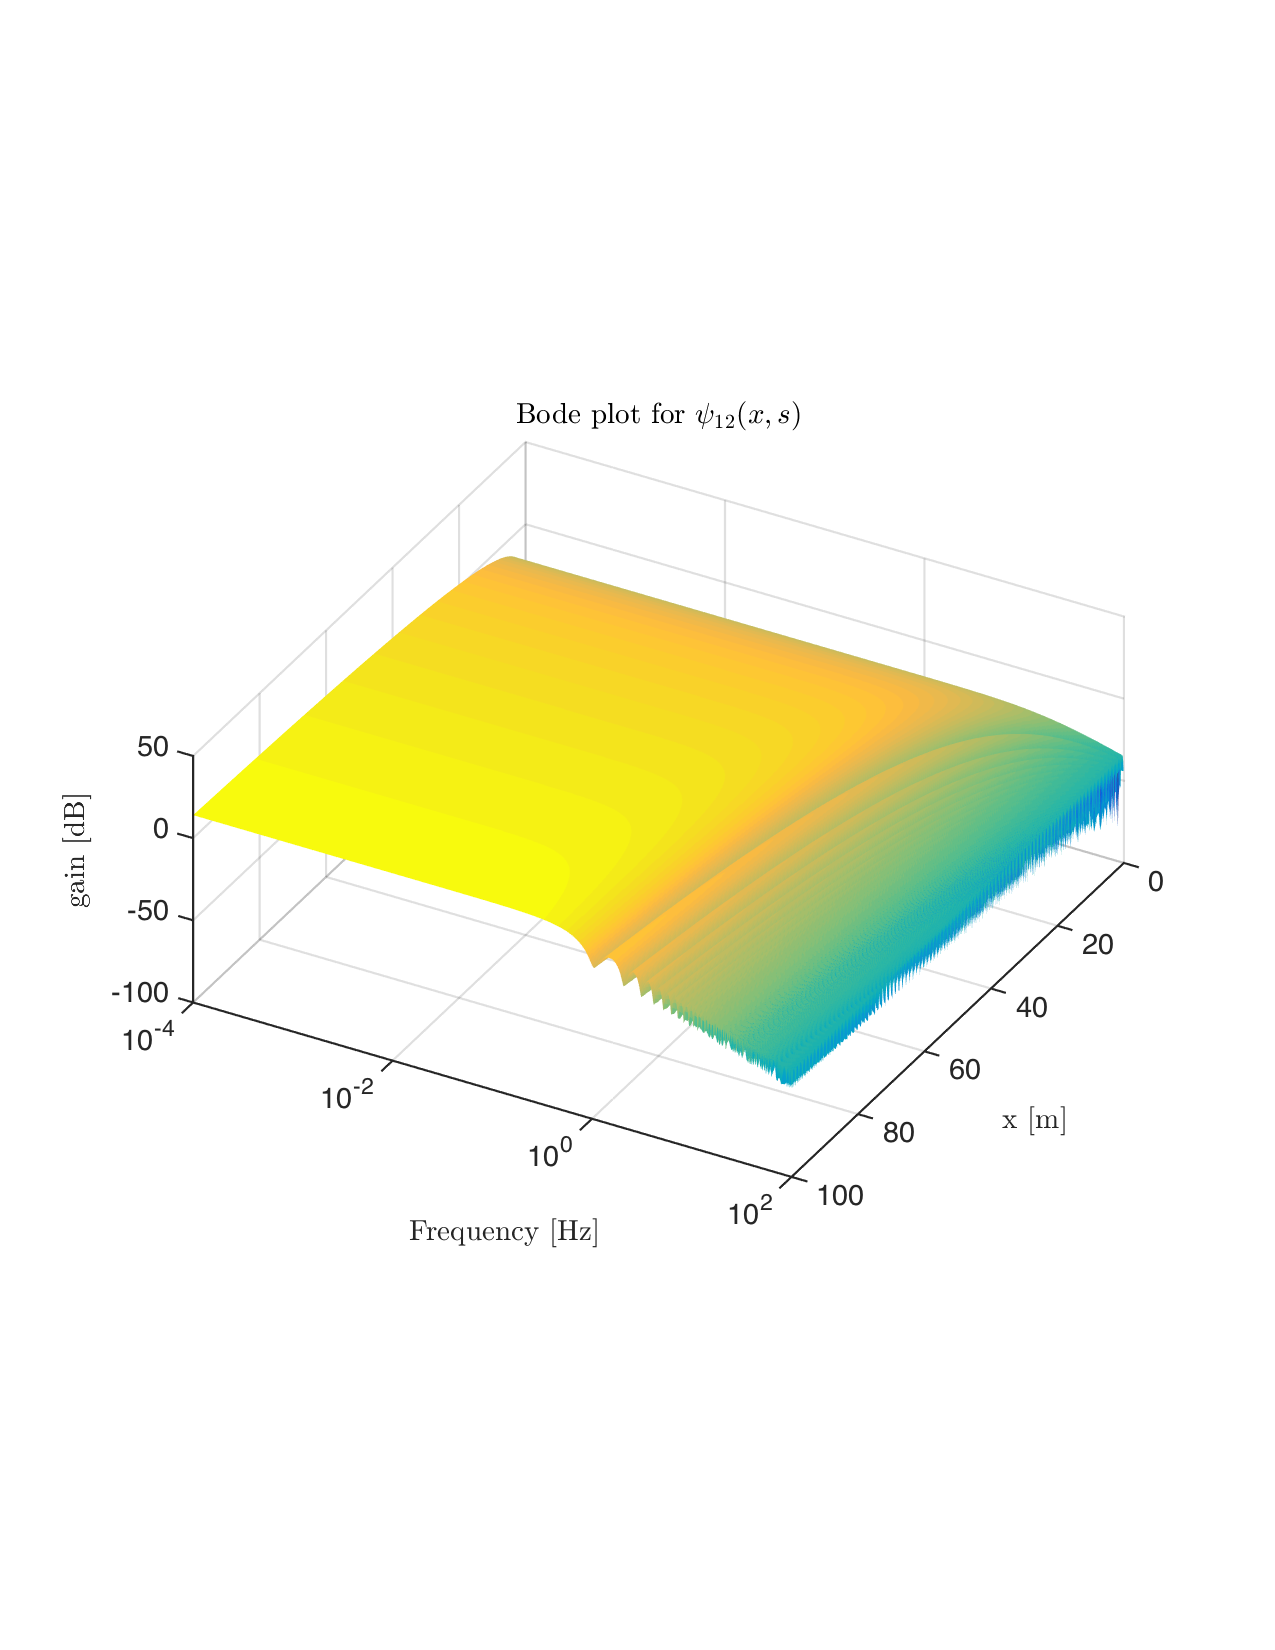
\includegraphics[trim = 0mm 60mm 0mm 60mm, width = 3.9cm]{distr_psi_12}
\tabularnewline
$\psi_{11}(x,s)$.
&
$\psi_{12}(x,s)$.
\tabularnewline
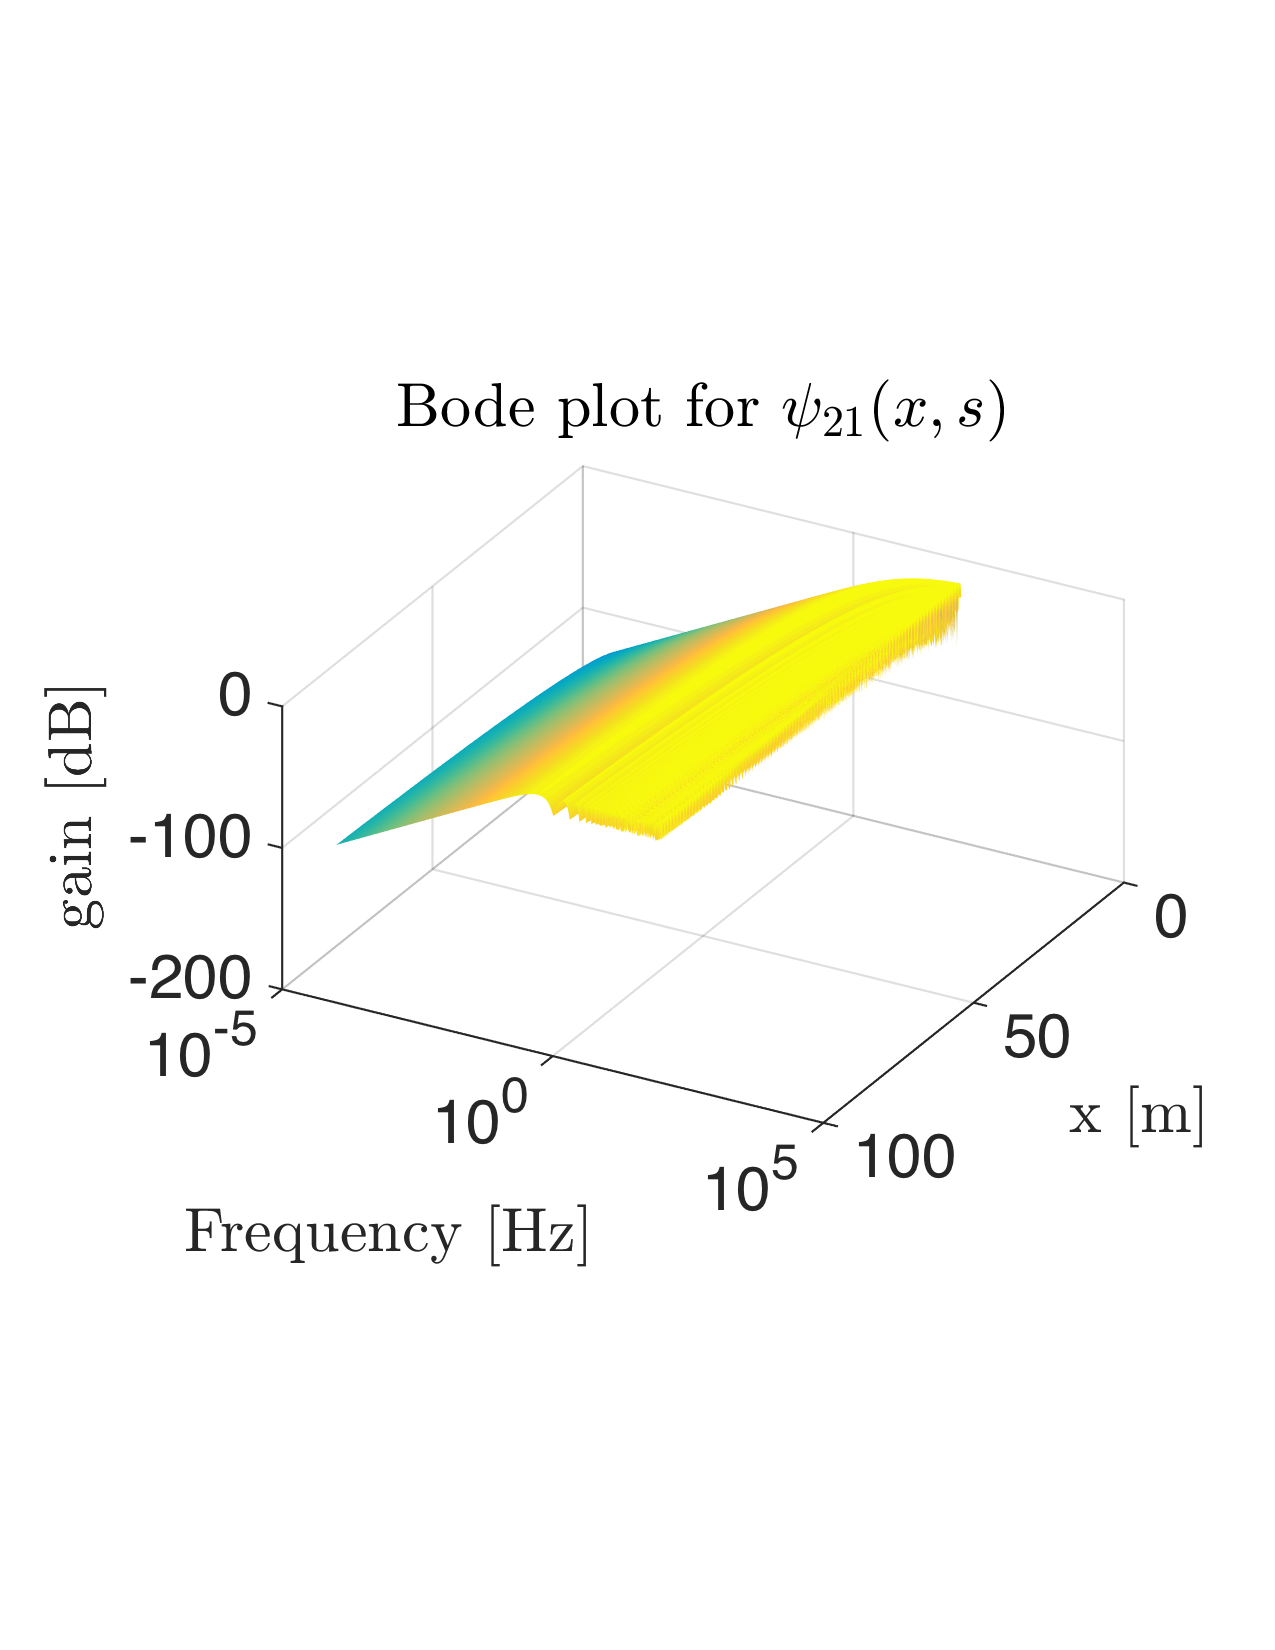
\includegraphics[trim = 0mm 60mm 0mm 60mm, width = 3.9cm]{distr_psi_21}
&
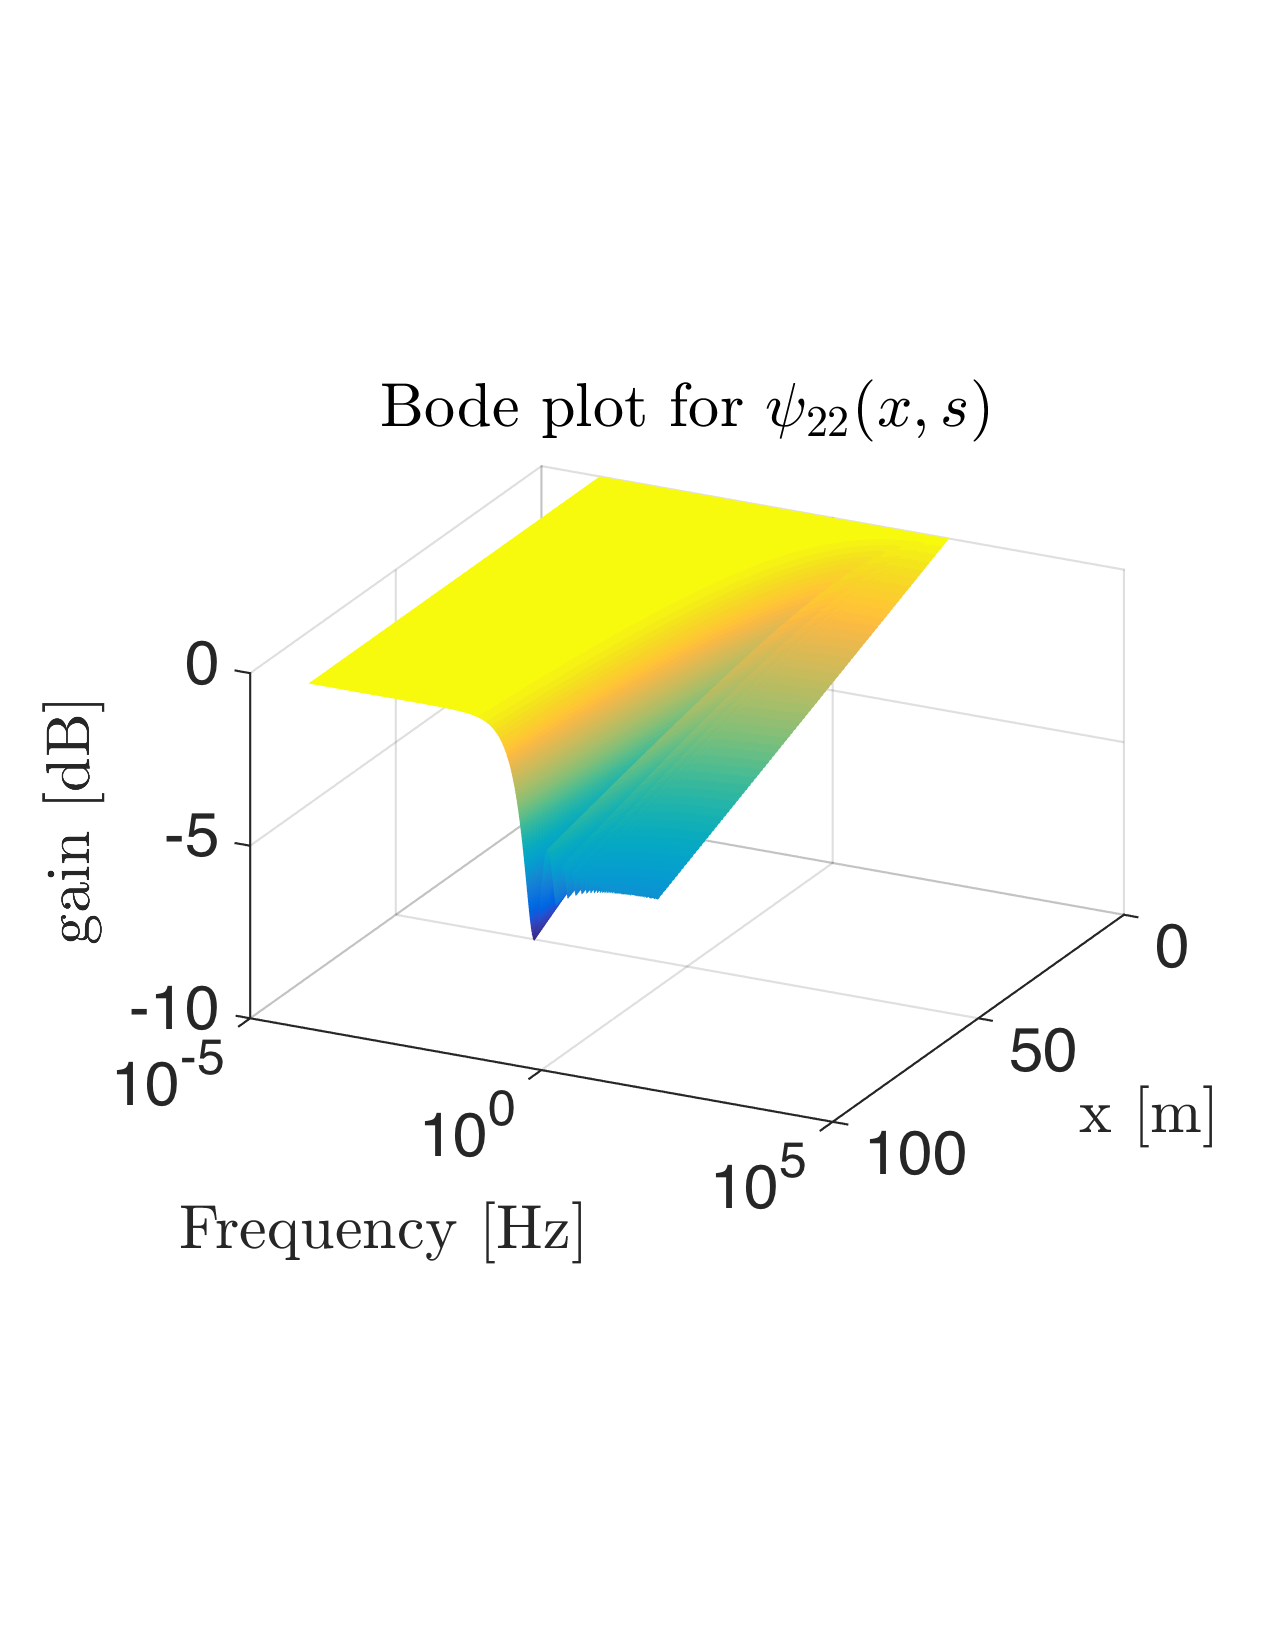
\includegraphics[trim = 0mm 60mm 0mm 60mm, width = 3.9cm]{distr_psi_22}
\tabularnewline
$\psi_{21}(x,s)$.
&
$\psi_{22}(x,s)$.
\end{tabular}
\caption{Spatial magnitude Bode plots for physical variables in free-flow regime ($\left|\alpha\right| = $ 0.53 Hz)\label{fig:Magn_spatial_physx}}
\end{figure}

For transfer functions featuring {\footnotesize$1 - e^{-\frac{x}{\lambda_{1} \tau \alpha} \left(s + \alpha \right)}$} as a factor (that is to say $\psi_{12}$, and $\psi_{21}$) one can observe in the corresponding Bode plots that the value of the log-gain in high frequency tends to vary very sharply. Indeed, with $s = jw$,
{\footnotesize
$
\left| 
	1 - e^{-\frac{x}{\lambda_{1} \tau \alpha} \left(s + \alpha\right)}
\right| = 
e^{-\frac{x}{\lambda_{1} \tau}}
\sqrt{
	\left(
		e^{\frac{x}{\lambda_{1}\tau}} 
		-
		\cos\left(\frac{w}{\lambda_{1} \tau \alpha} x\right)
	\right)^{2}
	+
	\sin^{2}\left( \frac{w}{\lambda_{1} \tau \alpha} x \right)
}
$
}. Therefore, if the spatial pseudo-period {\footnotesize$\tilde{L}=\frac{2\pi}{w} \lambda_{1} \tau \left|\alpha\right|$} is low enough, near zero values appear when $x$ is a multiple of $\tilde{L}$. This explains the irregular shape of the distributed Bode plots of $\phi_{21}$, $\psi_{12}$, and $\psi_{21}$ for frequencies {\footnotesize$w \gg 2 \pi \frac{\lambda_{1} \tau \left|\alpha\right|}{L} = 6.53$} Hz. This does not impact the stability of the system. Bode plots only look irregular about such points because of the logarithmic scale.\\

\subsubsection{Step responses}
We analyze the behavior of the system given step inputs {\footnotesize$\tilde{v}(0,t)=\bar{v}H(t)$} and {\footnotesize$\tilde{q}(0,t)=\bar{q}H(t)$}, where $H(\cdot)$ is the Heaviside function. The step responses can be explicitly computed from the spectral responses, let {\footnotesize$H_1(t,x) = H\left(t-\frac{x}{\lambda_{1}}\right)$} and
{\footnotesize$H_2(t,x) = H\left(t - \frac{x}{\lambda_{2}} \right)$}:

{\footnotesize
\begin{align}
\tilde{v}(x,t) &= 
\bar{v}
e^{-\frac{x}{\lambda_{1}\tau}}H_1(t,x)
\notag\\
&\quad
+\bar{v}
e^{-\alpha \left(t - \frac{x}{\lambda_{2}} \right)}
	(H_2 - H_1)(t,x)
\notag \\
&\quad
- \dfrac{\bar{q}}{\rho^* \tau}
\left(
	e^{-\frac{x}{\lambda_{1}\tau}}H_1\left(t,x\right) 
	- H_2(t,x)
\right) 
\notag\\
&\quad
- \dfrac{\bar{q}}{\rho^* \tau} e^{-\alpha \left(t - \frac{x}{\lambda_{2}} \right)}
	(H_2 - H_1)(t,x)\\
\tilde{q}(x,t) &= \bar{v} \rho^*\tau \alpha e^{-\alpha \left(t - \frac{x}{\lambda_{2}} \right)}
	(H_1 - H_2)(t,x)
\notag \\
&\quad+ 
\bar{q}
H_2(t,x)
\notag\\
&\quad
+
\bar{q}
e^{-\alpha \left(t - \frac{x}{\lambda_{2}} \right)}
	(H_1 - H_2)(t,x)	
\end{align}
}

With this set of time domain expressions, we can see that a cone of exponentially growing speed and flow linearization errors generally appears between the characteristic lines corresponding to $\lambda_{1}$ and $\lambda_{2}$. This is caused by $\alpha$ being negative in the free flow regime and means that, in this region of the domain $\left[0,T\right] \times \left[0,L\right]$, the $\left(v,q\right)$ state of the linearized system can diverge exponentially fast from the linearization point. This is consistent with the observations in \cite{PhysRevLett.79.4030} where small local perturbations occurring in free-flow regime can cause traffic to transition durably to the congested regime.

\begin{figure}
\begin{centering}
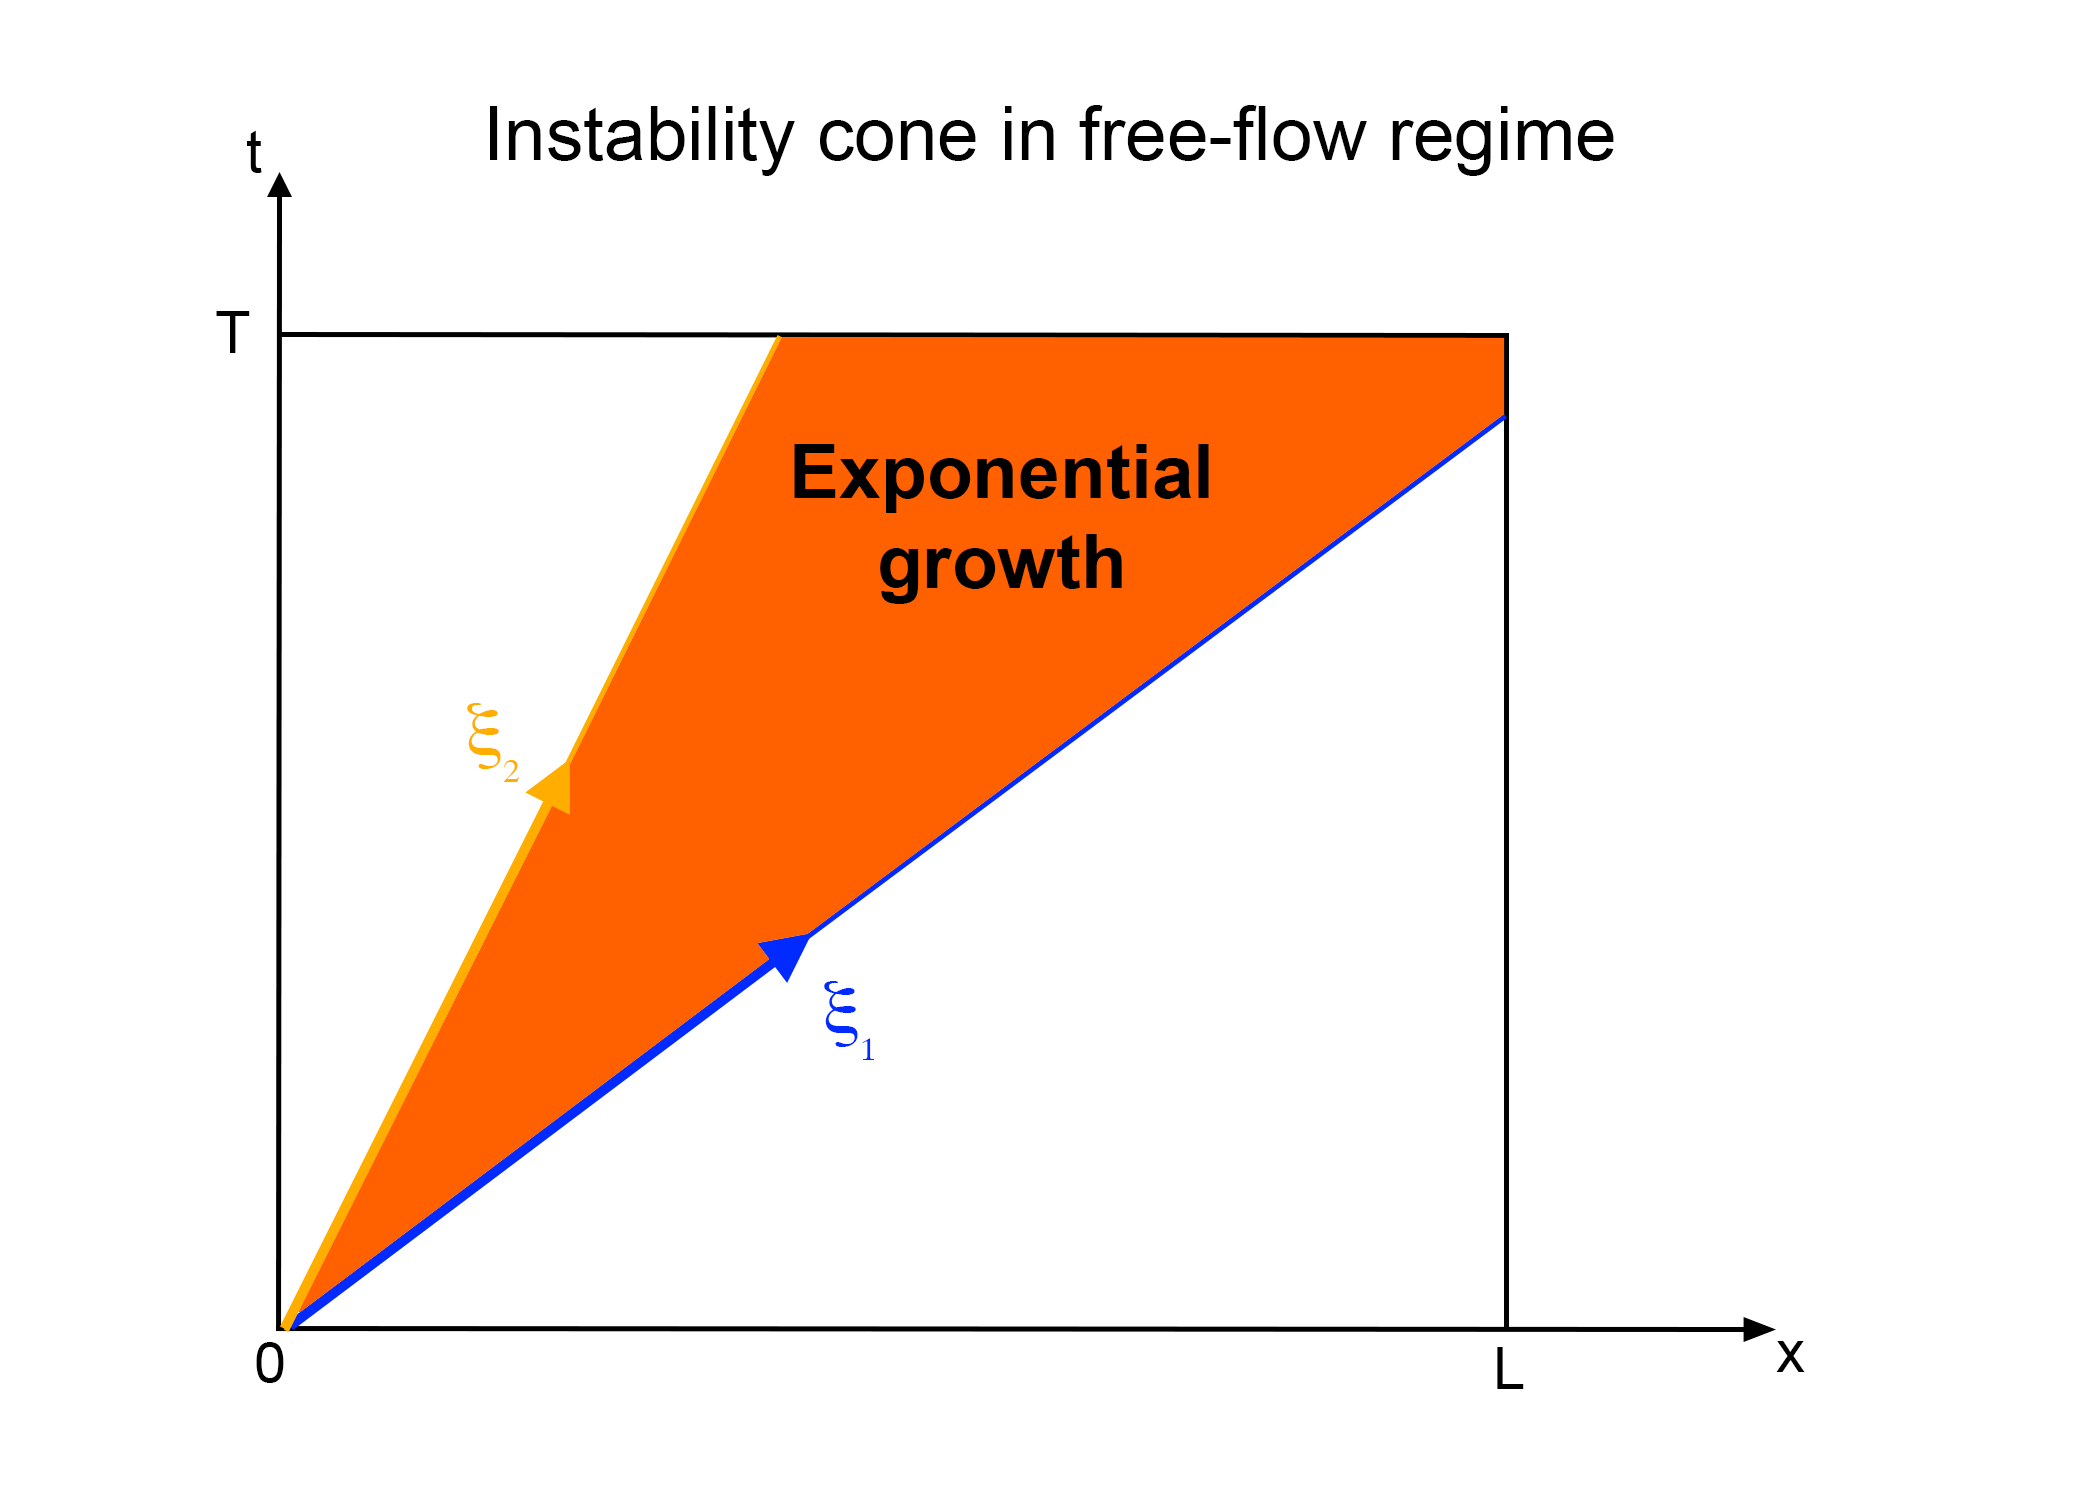
\includegraphics[width=4cm]{Exp-growth}
\par\end{centering}
\protect\caption{Exponential growth cone appearing in the free-flow regime for $v$ and $q$.\label{Exp-growth}}
\end{figure}

\subsection{Congested regime ($F>1$)}
Considering the system in congested regime, using \eqref{TFRiemann} we can write
{\footnotesize
$\label{vqcongested}
\begin{pmatrix}
	\hat{\xi_{1}}(x,s)\\
	\hat{\xi_{2}}(x,s)
\end{pmatrix} = 
\Gamma(x,s)
\begin{pmatrix}
	\hat{\xi_{1}}\left(0,s\right)\\
	\hat{\xi_{2}}\left(L,s\right)
\end{pmatrix}
$
}
with 
{\footnotesize
\begin{subequations}
\begin{align}
\gamma_{11}\left(x,s\right)&=
e^{-\frac{x}{\lambda_{1}}\left(s+\frac{1}{\tau}\right)} , \\
\gamma_{12}\left(x,s\right)&=0, \\
\gamma_{21}\left(x,s\right)&=
\frac{\lambda_{1} \alpha e^{-\frac{x}{\lambda_{1}} \left( s + \frac{1}{\tau} \right)}}
{\lambda_{2}\left(s + \alpha\right)}
\left(
	1 -
	e^{-\frac{\left(L - x\right)
		}{
		\lambda_{1}\tau\alpha
		}
		\left(s+\alpha\right)
		}
\right)
, \\
\gamma_{22}\left(x,s\right)&=e^{\frac{s\left(L-x\right)}{\lambda_{2}}}.
\end{align}
\end{subequations}
}

\subsubsection{Transfer functions for physical variables in congested regime}
In congested regime, the boundary conditions used to control the system are $\hat{\xi}_{1}\left(0,\cdot\right)$ and $\hat{\xi}_{2}\left(0,\cdot\right)$. By linearity of the Laplace transform
{\footnotesize
$\hat{\xi_{1}}\left(0,s\right) = 
\frac{
	\rho^{*}\lambda_{2}
}{
	\lambda_{1} - \lambda_{2}
} 
\hat{v}\left(0,s\right)
+
\hat{q}\left(0,s\right)
$.}
Therefore, as
{\footnotesize
$\hat{\xi_{2}}\left(0,s\right) =
\gamma_{21}\left(0,s\right)
\hat{\xi_{1}}\left(0,s\right)
+
\gamma_{22}\left(0,s\right)
\hat{\xi_{2}}\left(L,s\right)$}
, we get
{\footnotesize
$\hat{\xi_{1}}\left(0,s\right) =
\frac{1}{d\left(s\right)}
\hat{q}\left(0,s\right)
+
\frac{n\left(s\right)}{d\left(s\right)}
\hat{v}\left(L,s\right)
$}
where
{\footnotesize
$d\left(s\right) = 1 - \frac{\lambda_{2}}{\lambda_{1}}\gamma_{21}\left(0,s\right)$}
and
{\footnotesize$n\left(s\right) = \frac{\rho^{*} \lambda_{2}}{\lambda_{1} - \lambda_{2}} \gamma_{22}\left(0,s\right)$}. The $\left(v,q\right)$ system has only two degrees of freedom. Therefore we consider that the only inputs to the system are $q\left(0,\cdot\right)$ and $v\left(L,\cdot\right)$. At the boundary, $v\left(0,\cdot\right)$ is then completely determined and can be interpreted as an output of the system. The corresponding transfer equation is
{\footnotesize
\begin{equation}
\begin{pmatrix}
	\hat{v}\left(x,s\right)
	\\
	\hat{q}\left(x,s\right)
\end{pmatrix}
=
\underset{\Theta\left(x,s\right)}{
\underbrace{
R^{-1}\Gamma\left(x,s\right)
\begin{pmatrix}
	\frac{n\left(s\right)}{d\left(s\right)}
		&
	\frac{1}{d\left(s\right)}	
	\\
	\frac{\rho^{*}\lambda_{1}}{\lambda_{1} - \lambda_{2}}
		&
	0
\end{pmatrix}
}
}
\begin{pmatrix}
	\hat{v}\left(L,s\right)
	\\
	\hat{q}\left(0,s\right)
\end{pmatrix}
\end{equation}
}
where
{\footnotesize
\begin{subequations}
\begin{align}
\theta_{11}\left(x,s\right) &=
\frac{
	\alpha 
		e^{
			-\frac{x}{\tau\lambda_{1}}
		}
		e^{
			-\frac{s}{\lambda_{1}}
				\left(
					x - L\frac{\lambda_{1}}{\lambda_{2}}
				\right)	
		}
	+
	s 
		e^{-\frac{s}{\lambda_{2}}\left(x - L\right)}
}{
	s
	+
	\alpha
	e^{-\frac{L}{\tau\lambda_{1}}}
	e^{
	-\frac{sL}{\lambda_{1}}
	\left(
		1 - \frac{\lambda_{1}}{\lambda_{2}}
	\right)
	}
}
,\\
\theta_{12}\left(x,s\right) &=
\frac{
	e^{-\frac{L}{\tau\lambda_{1}}}
	e^{-\frac{s}{\lambda_{2}}
		\left(
			x - L
				\left(1 - 
					\frac{\lambda_{2}}{\lambda_{1}}
				\right)
		\right)
	}
	-
	e^{-\frac{x}{\tau\lambda_{1}}}
	e^{-\frac{sx}{\lambda_{1}}}
}
{
	\rho^{*}\tau
	\left(
		s
		+
		\alpha
		e^{-\frac{L}{\tau\lambda_{1}}}
		e^{
			-\frac{sL}{\lambda_{1}}
			\left(
				1 - \frac{\lambda_{1}}{\lambda_{2}}
			\right)
			}
	\right)
},\\
\theta_{21}\left(x,s\right) &=
\rho^{*}\tau\alpha s
\frac{
	e^{-\frac{s\left(x-L\right)}{\lambda_{2}}}
	-
	e^{-\frac{x}{\tau\lambda_{1}}}
	e^{-\frac{s}{\lambda_{1}}
		\left(
			x - L\frac{\lambda_{1}}{\lambda_{2}}
		\right)
	}
}{
	s
	+
	\alpha
	e^{-\frac{L}{\tau\lambda_{1}}}
	e^{
	-\frac{sL}{\lambda_{1}}
	\left(
		1 - \frac{\lambda_{1}}{\lambda_{2}}
	\right)
	}
},\\
\theta_{22}\left(x,s\right) &=
\frac{
	\alpha
	e^{-\frac{L}{\tau\lambda_{1}}}
	e^{-\frac{s}{\lambda_{2}}
		\left(
			x - L
				\left(
				1 - \frac{\lambda_{2}}{\lambda_{1}}
				\right)
		\right)
	}
	+
	s
	e^{-\frac{x}{\tau\lambda_{1}}}
	e^{-\frac{sx}{\lambda_{1}}}
}{
	s
	+
	\alpha
	e^{-\frac{L}{\tau\lambda_{1}}}
	e^{
	-\frac{sL}{\lambda_{1}}
	\left(
		1 - \frac{\lambda_{1}}{\lambda_{2}}
	\right)
	}
}
.
\end{align}
\end{subequations}
}

\subsubsection{Low frequency approximation for physical variables in congested regime}
We derive approximate expressions in the frequency domain for the transfer functions above when $\left|s\right|\ll\left|\alpha\right|$:
{\footnotesize
\begin{subequations}
\begin{align}
\theta_{11}\left(x,s\right) &\simeq
e^{\frac{s\left(L-x\right)}{\lambda_{2}}}
e^{\frac{L-x}{\tau\lambda_{1}}},\\
\theta_{12}\left(x,s\right) &\simeq
\frac{1}{\rho^{*}\tau\alpha}
e^{-\frac{sx}{\lambda_{1}}}
\left(
	1 - e^{\frac{L-x}{\tau\lambda_{1}}}
\right),\\
\theta_{21}\left(x,s\right) &\simeq
s \rho^{*}\tau
e^{\frac{s\left(L-x\right)}{\lambda_{2}}}
e^{\frac{L}{\tau\lambda_{1}}}
\left(
	1 - e^{-\frac{x}{\tau\lambda_{1}}}
\right),\\
\theta_{22}\left(x,s\right) &\simeq
e^{-\frac{sx}{\lambda_{1}}}.
\end{align}
\end{subequations}
}

With such expressions, interpreting the approximate transfer functions in low frequencies becomes fairly easy in terms of information propagating from the boundary conditions into the resolution domain with two different speeds: $\lambda_1$ and $\lambda_2$. Once again, one can notice distributed gain components with characteristic distance $\lambda_1 \tau$. A derivator component in $\theta_{21}$ relates $\hat{\xi}_2(x,s)$ to $\hat{\xi}_1(0,s)$.\\

\subsubsection{Bode plots for congested regime}
We use the same fundamental diagram as in the free-flow case. However the linearization point, $\rho^* = 0.08$ veh/m, corresponds to the congested region of the Greeshields diagram. We show the distributed Bode plots for the physical variables in Figure \ref{fig:Magn_spatial_physx_congested}. In that case, $\alpha =$ 0.05 Hz, which does correspond to a reasonable characteristic frequency for traffic modeling applications.

Similarly to the free-flow case, for high frequencies ($w \gg 2 \pi \frac{\lambda_{1} \tau \alpha}{L} = 0.13$ Hz) near zero values appearing with spatial periodicity $\frac{2 \pi}{w} \lambda_{1} \tau \alpha$ almost cancel out $\gamma_{21}$, $\theta_{12}$, and $\theta_{21}$. Such points only appear as irregularities in the Bode plots because the gain is computed on a logarithmic scale.\\

\begin{figure}
\centering
\begin{tabular}{cc}
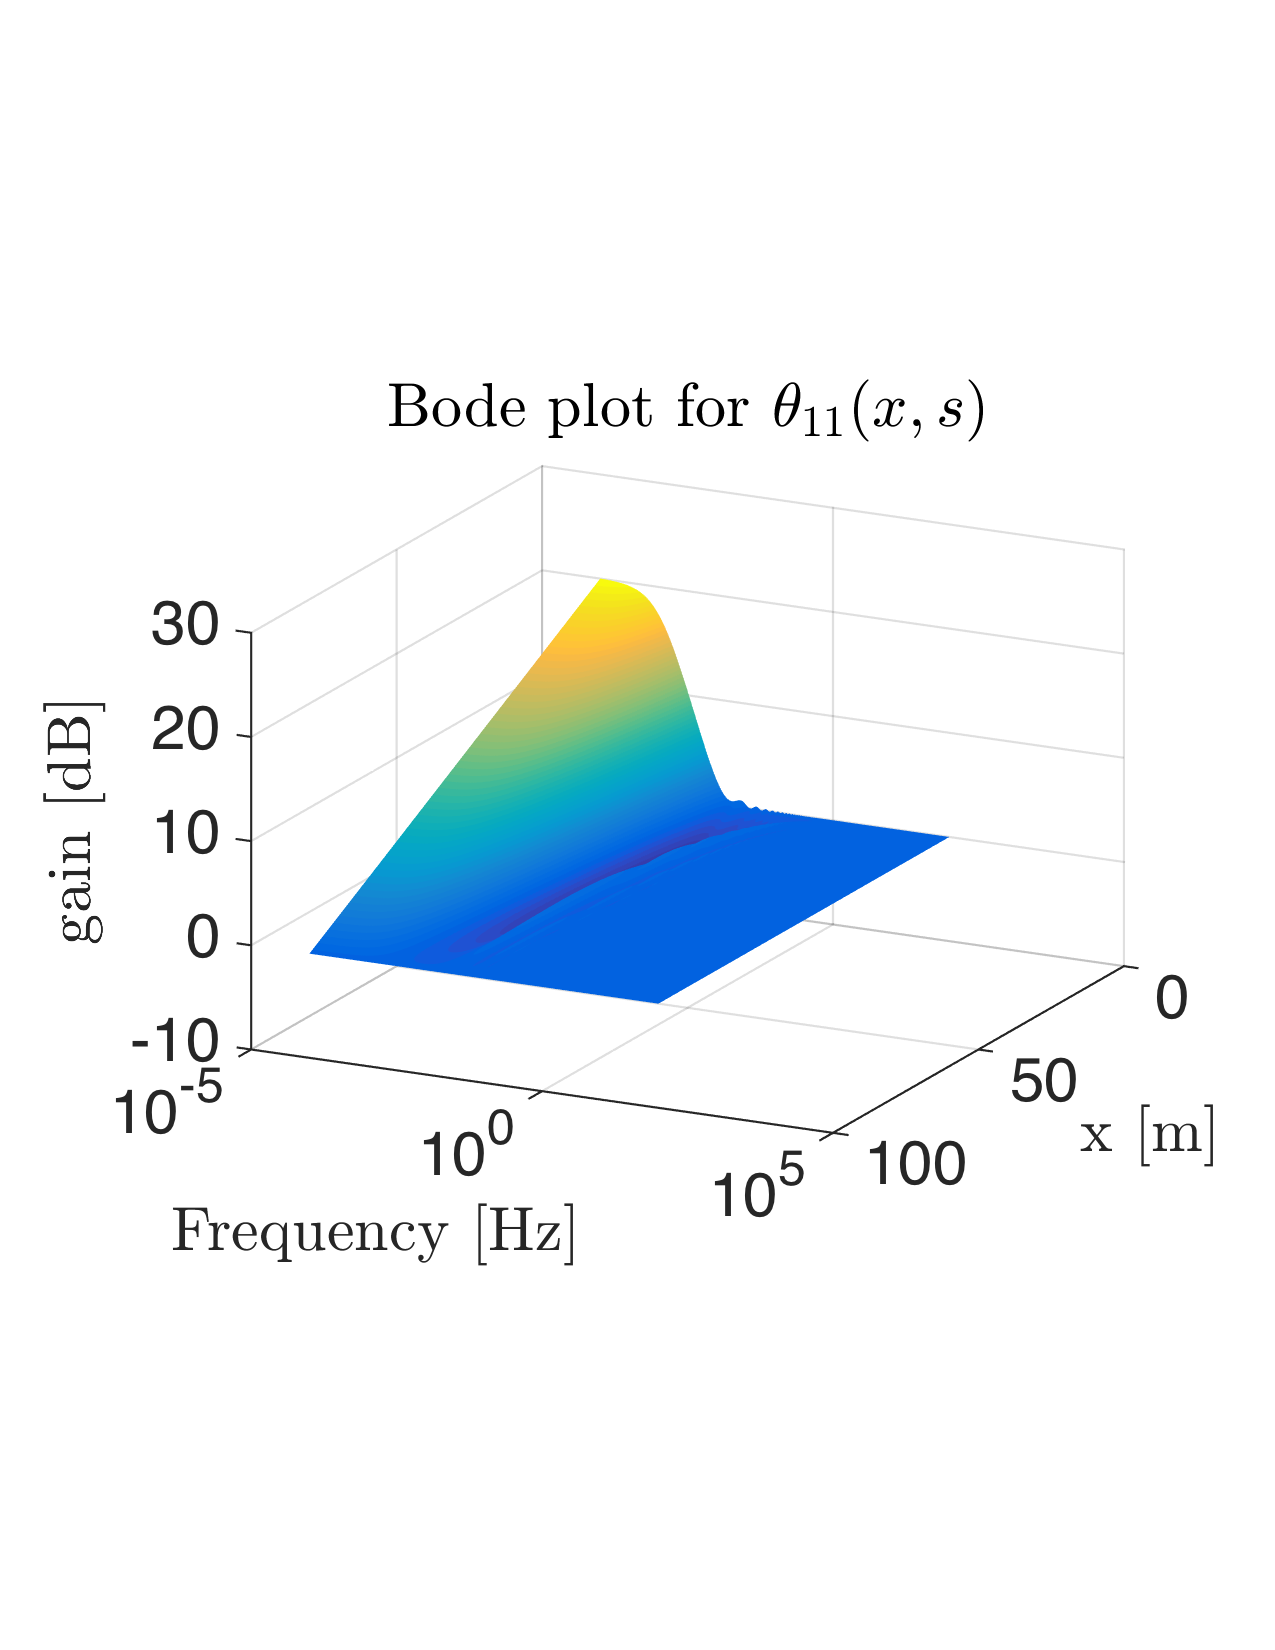
\includegraphics[trim = 0mm 60mm 0mm 60mm, width = 3.9cm]{distr_theta_11}
&
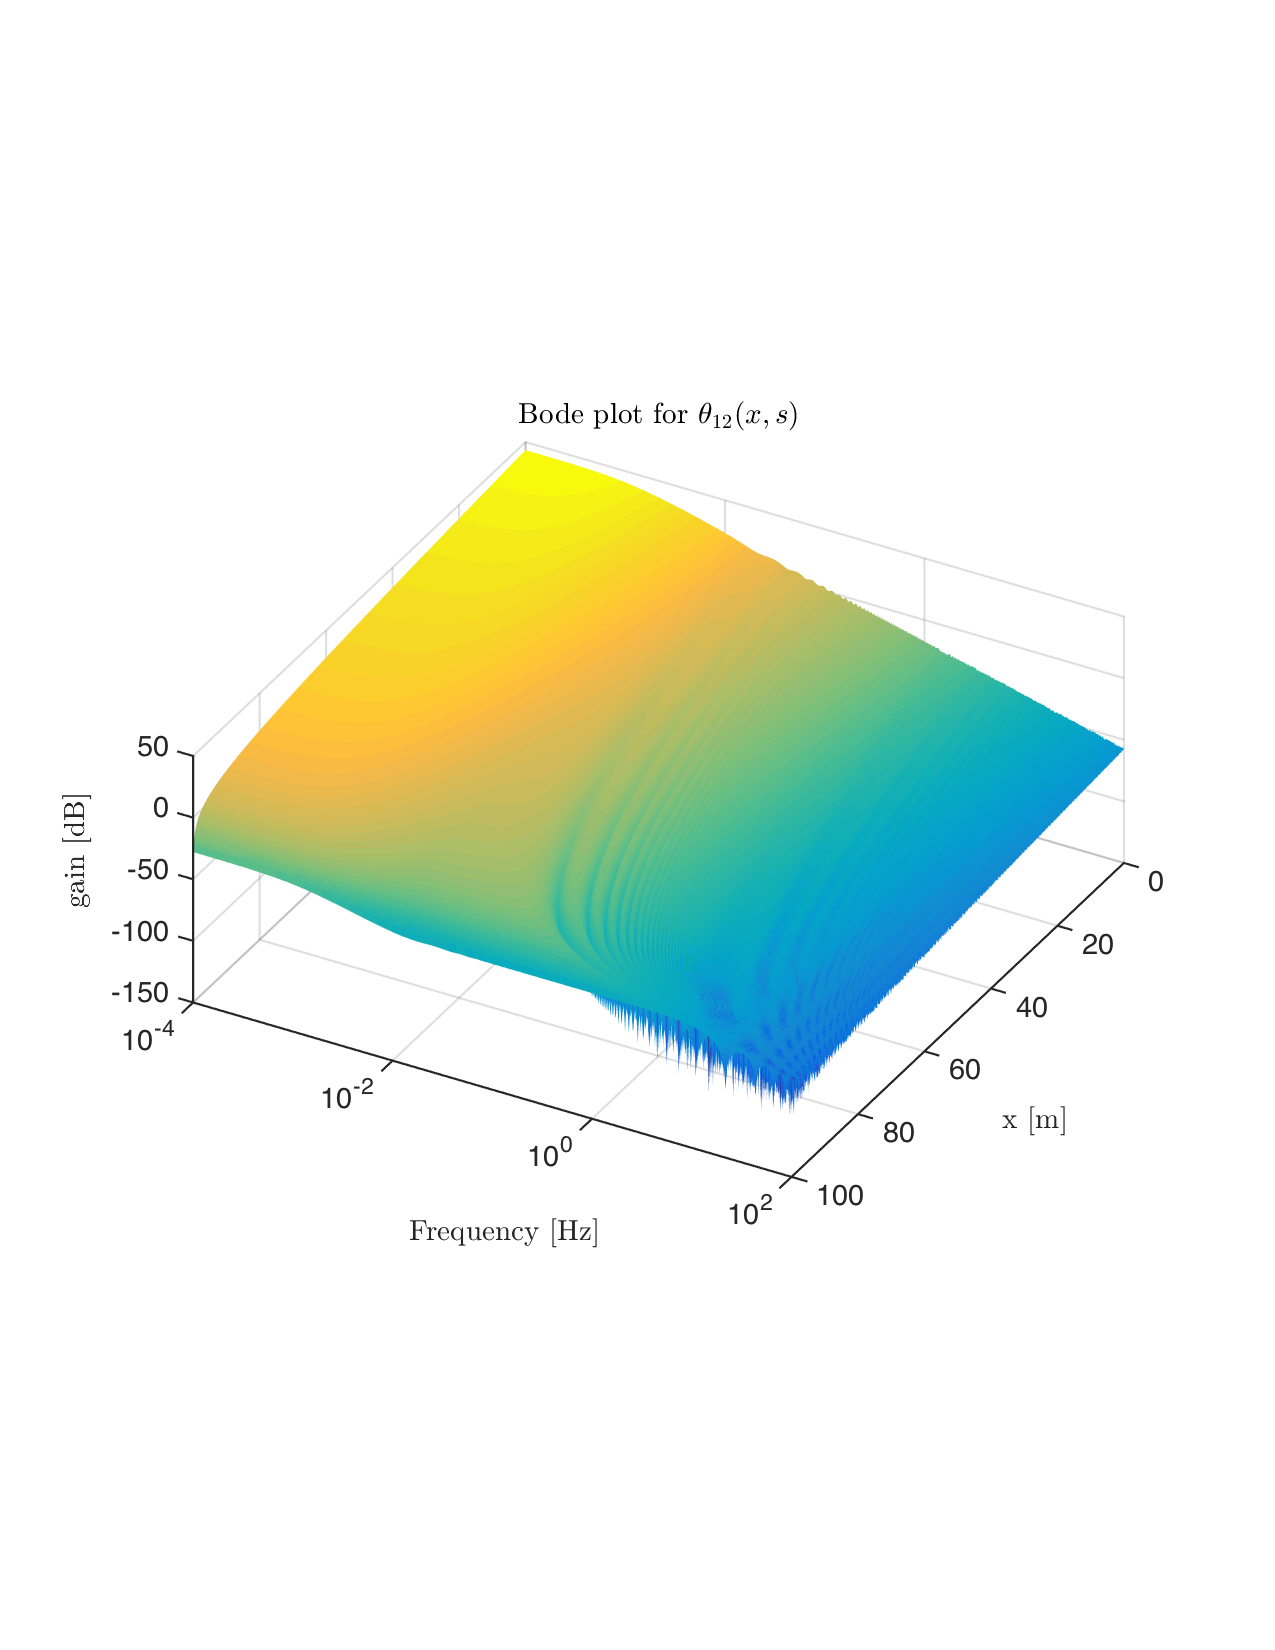
\includegraphics[trim = 0mm 60mm 0mm 60mm, width = 3.9cm]{distr_theta_12}
\tabularnewline
$\theta_{11}(x,s)$.
&
$\theta_{12}(x,s)$.
\tabularnewline
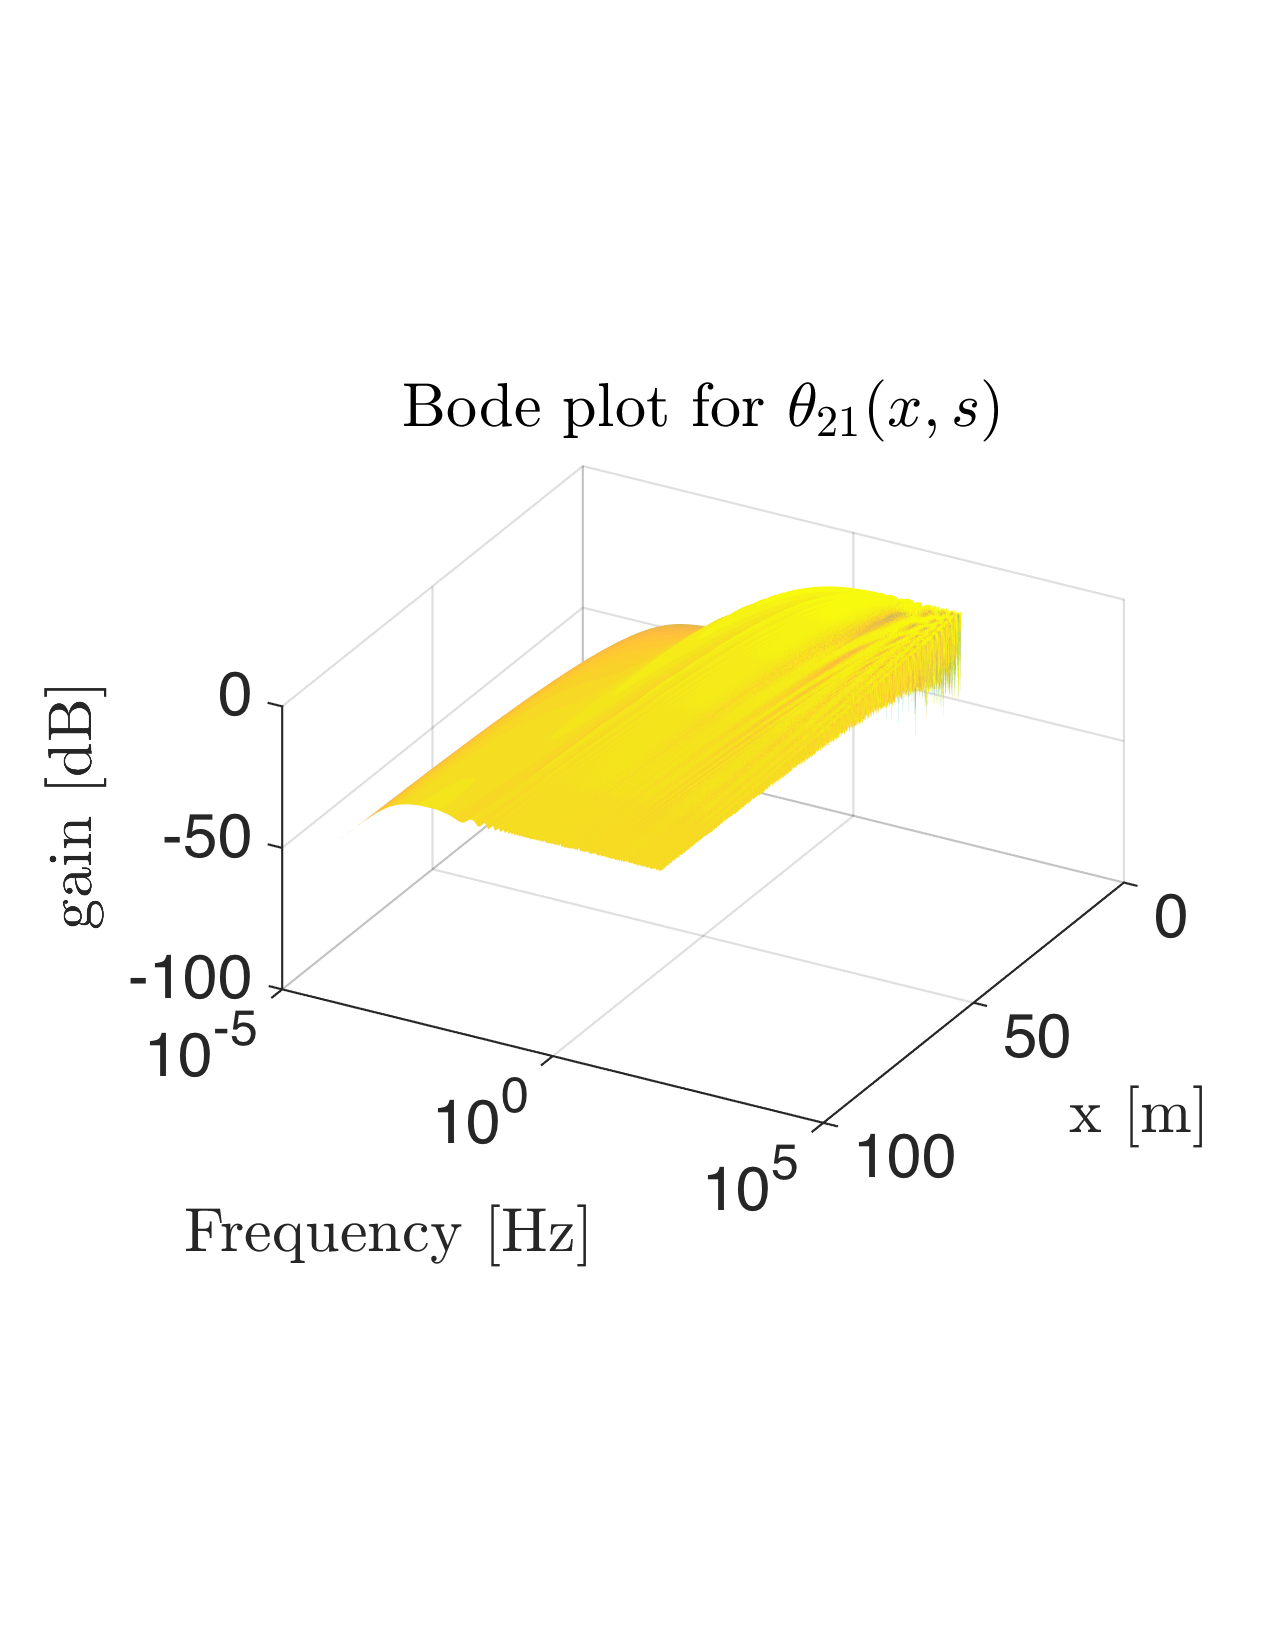
\includegraphics[trim = 0mm 60mm 0mm 60mm, width = 3.9cm]{distr_theta_21}
&
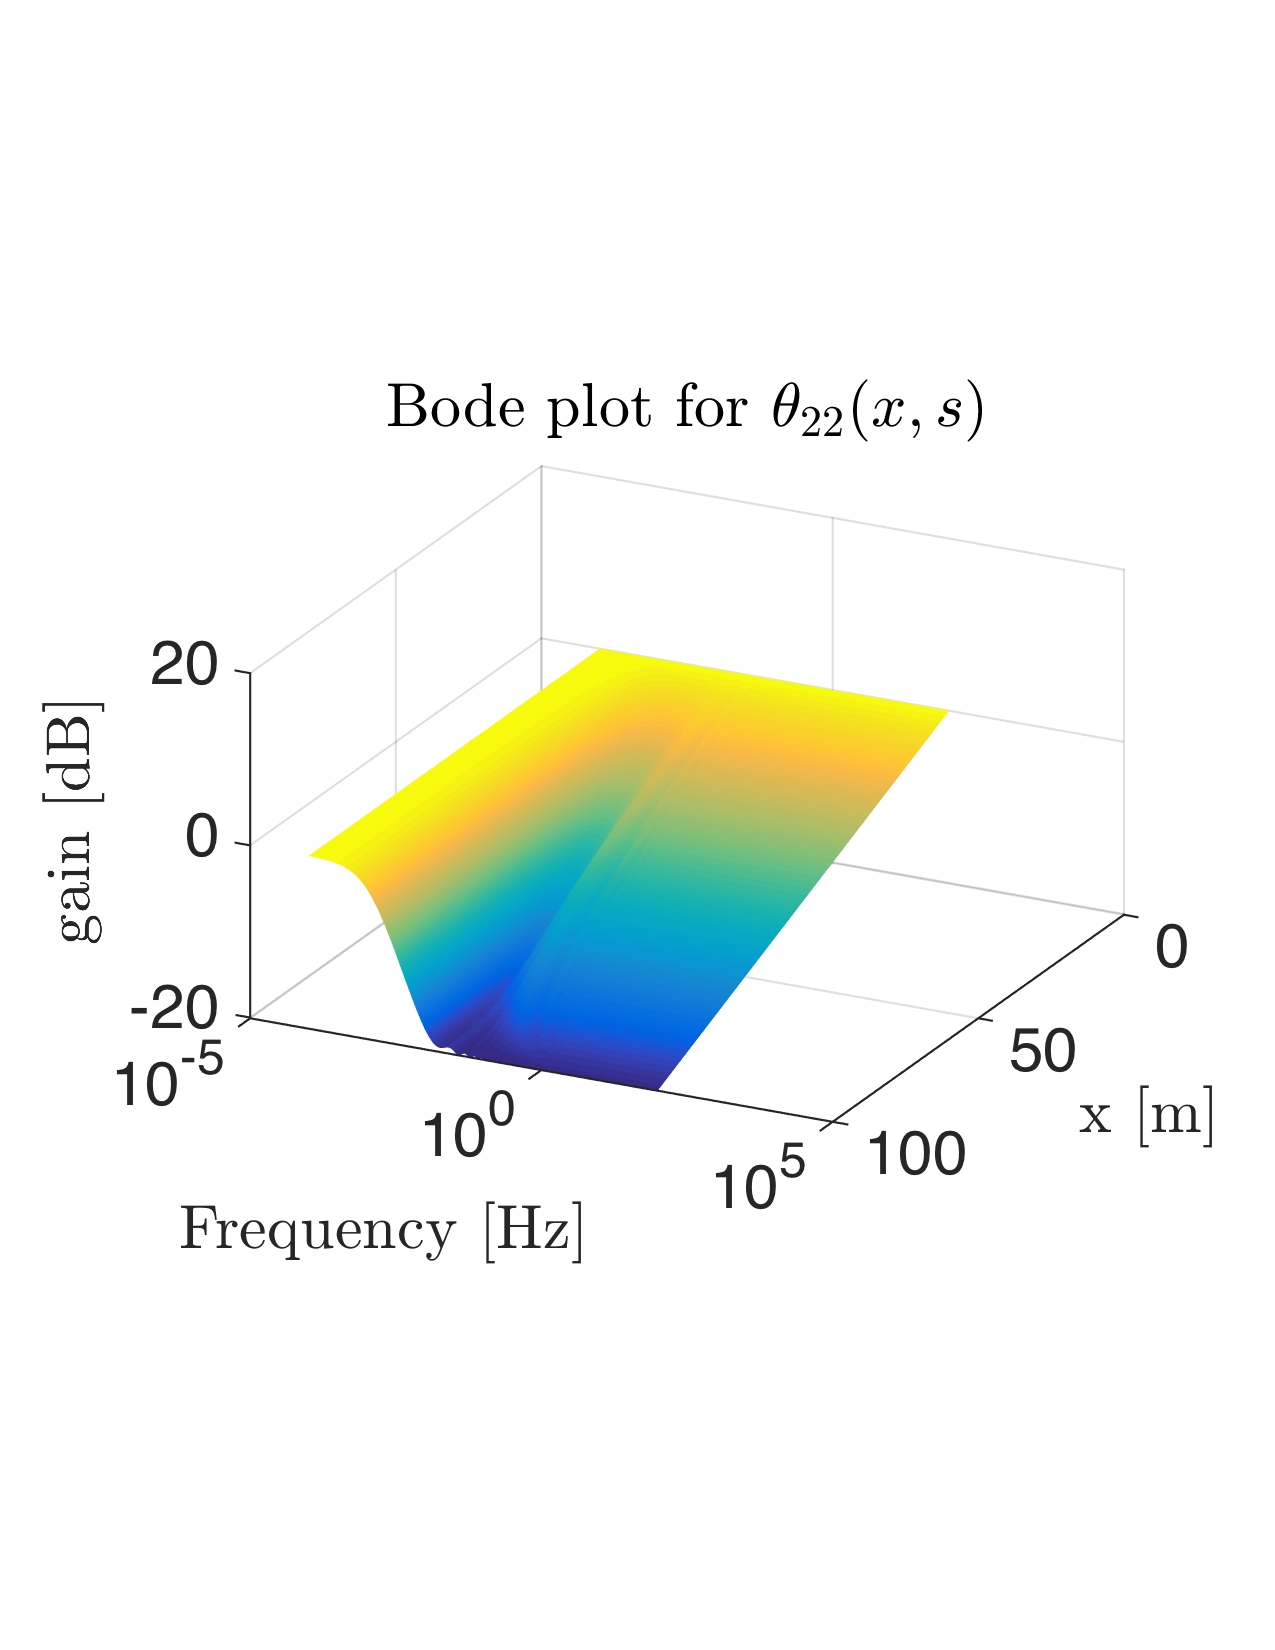
\includegraphics[trim = 0mm 60mm 0mm 60mm, width = 3.9cm]{distr_theta_22}
\tabularnewline
$\theta_{21}(x,s)$.
&
$\theta_{22}(x,s)$.
\tabularnewline
\end{tabular}
\caption{Spatial magnitude Bode plots for physical variables in congested regime ($\left|\alpha\right| = $ 0.05 Hz)\label{fig:Magn_spatial_physx_congested}}
\end{figure}

\subsubsection{Poles and BIBO stability of the system}
In order to practically assess the presence of poles, numerical search for roots of the denominator of the transfer functions has been conducted thanks to standard equation solvers. Once more $-\alpha$ is a solution and another one was found at $s=-0.0018$. They are both negative reals and therefore cannot make the system unstable. Although the solvers could have detected poles with a non zero imaginary part, none has been found. Holistic search for other poles should be conducted but is out of the scope of this article.


\section{Numerical validation}
Prior to using standard control theoretic techniques, it is necessary to assess how accurate the model is in its linearized form. This section compares the prediction of the linearized equations with actual flow and velocity data gathered from the well-known NGSIM data set.


\subsection{Data source: NGSIM trajectories}
We use the NSGIM trajectory data set for a uniform 200 meter long section of the US-101 highway where no ramps perturb the homogeneity of traffic. The set gathers 45 minutes worth of trajectories of vehicles sampled with a 10 Hz frequency in the area described in Figure \ref{fig:NGSIM-trajectories}.

\begin{figure}
\centering
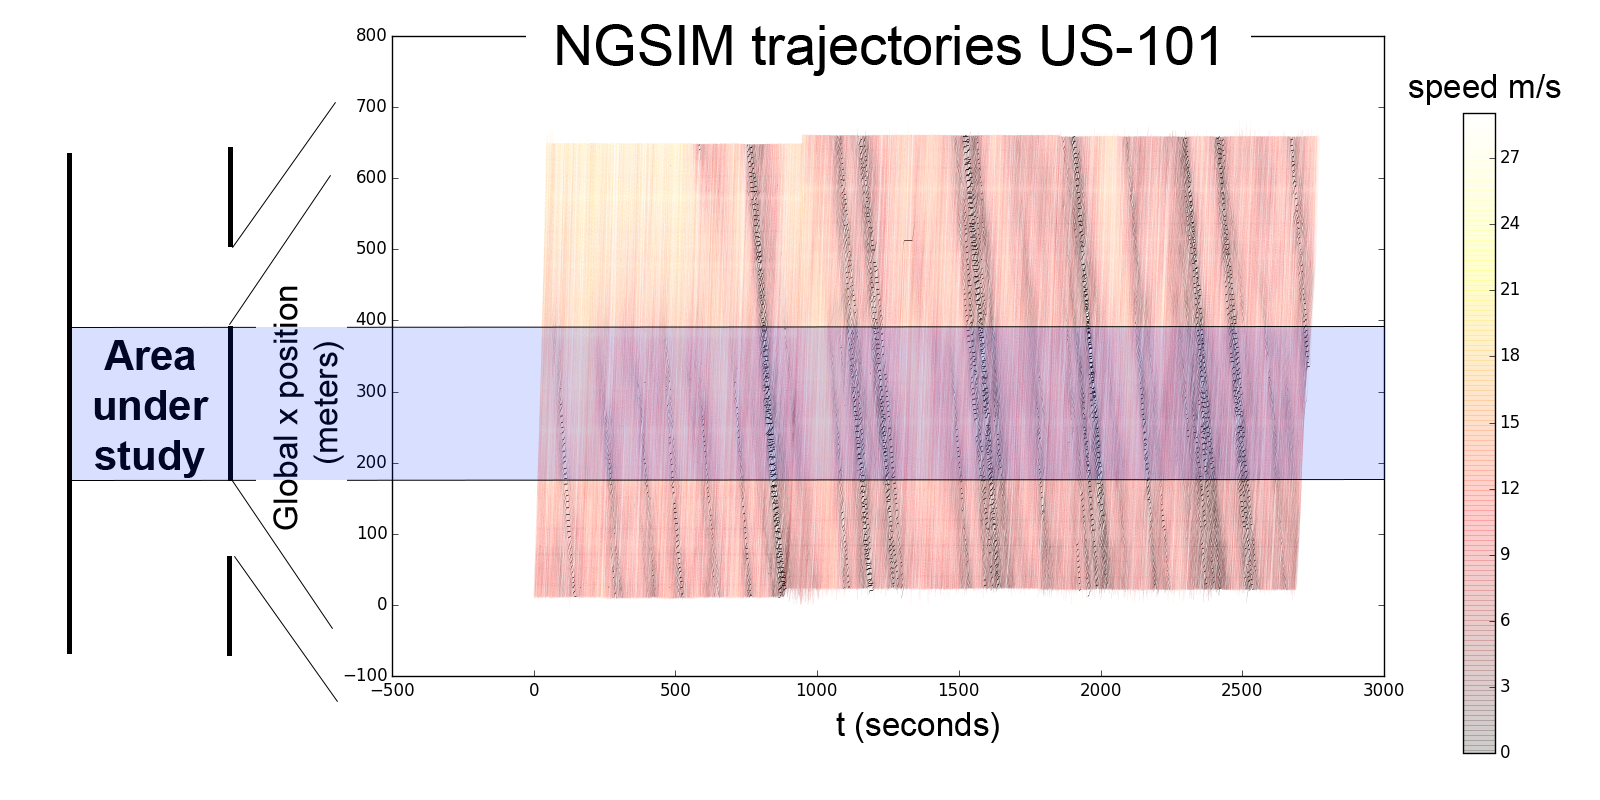
\includegraphics[width=7cm]{US-101_all_traj_low_res_mod}
\protect\caption{NGSIM trajectories. Color represents the measured speed of each
car in m/s.}
\label{fig:NGSIM-trajectories}
\end{figure}



\subsection{Reconstructing $(v,q)$ maps from NGSIM trajectories}

The NGSIM data set does not directly provide the values $v(t,x)$ and $q(t,x)$ in the resolution domain $\left[0,T\right]\times\left[0,L\right]$. To obtain macroscopic quantities out of the microscopic measurements, we follow the approach devised in \cite{edie1963discussion} and divide the space-time grid into rectangular cells. This operation groups corresponding data points into cells, then estimating the quantities of interest in each cell, it was for example used in \cite{Piccoli201532}. The full estimation procedure is described in the appendix attached. It is validated by confronting two vehicular flow estimates obtained by radically different techniques. They both correspond throughout the estimated speed-flow map.\\

\subsubsection{Calibration of $\lambda_{1}$ and $\lambda_{2}$, linearization point}
In Section \ref{ARZSection}, we found that $\lambda_{1}$ is exactly $v^*$ and $\lambda_{2}$ is the slope of the fundamental diagram at $v^*$. Thus to calibrate the eigenvalues we must find the linearization point. Note the dataset used corresponds only to the congested regime and the fundamental diagram is almost affine. The estimator, $\widehat{\lambda}_1=\widehat{v}^*$ is chosen as the empirical mean of $\widehat{v}$. To estimate $\lambda_{2}$, we fit a linear model $\widehat{q}=b_{1}\widehat{\rho}+b_{0}+\varepsilon$ with an ordinary least squares procedure, where $\varepsilon$
represents the noise in the model that would ideally be centered,
homoschedastic, and uncorrelated but is not practically. Then $\widehat{\lambda}_{2}=\widehat{b}_{1}$ and we take $\widehat{q}^*$ as the empirical average of $\widehat{q}$. The ratio of $\widehat{q}^*$ and $\widehat{v}^*$ gives the estimate $\widehat{\rho}^*$.
The empirical results are presented in Figure \ref{fig:Calibration-of-eigen-values}. The determination coefficient is poor but can be improved by filtering out outliers and gathering more data. Further work should turn this rather heuristic method for estimating parameters into a fully justified statistical procedure.

\begin{figure}[H]
\centering
\includegraphics[width=5cm]{\string"Fundamental_diagram_fitting_n_80\string".png}
\protect\caption{Calibration of $\lambda_{1}$ and $\lambda_{2}$. The circle denotes the linearization point. The affine model used to estimate $\lambda_{2}$ and the linearization point is also plotted. The estimates are: $\widehat{\lambda}_{1}=8.96$ m/s, $\widehat{\lambda}_{2}=-4.37$ m/s, $\widehat{\rho}^{*}=0.049$ veh/m, $\widehat{v}^{*}=8.96$ m/s, $\widehat{q}^{*}=0.44$ veh/s, with $r^{2}=0.48$. The characteristic frequency of the system is $\widehat{\alpha} = 8.37\times10^{-3}$ Hz. Its order of magnitude does correspond to practical traffic flow modeling.}
\label{fig:Calibration-of-eigen-values}
\end{figure}

\subsection{Verification of the spectral form}
In this section we demonstrate the performance of the spectral form as a prediction tool using the time domain responses derived from the transfer functions above and FFT. Since we are working with a linearized system, we can decompose boundary conditions then add predicted values inside the domain $\left[0,T\right]\times\left[0,L\right]$. Fourier decomposition of boundary conditions is here extremely accurate as the median relative errors for the interpolation of the values of $\xi_{1}\left(x=0, \cdot \right)$ and $\xi_{2}\left(x=L, \cdot \right)$ are respectively $2\%$ and $3\%$.\\

\subsubsection{Simulated maps}
Since the spectral form presents information in the diagonalized basis, we need a conversion before we can compare the simulated results to the values estimated from the dataset. It takes into account both the fact that the linearized equation are based on deviations of $v$ and $q$ from the linearization point and the change of basis that is necessary to work with Riemann invariants. The inverse of this affine transformation yields in return predicted quantities for the physical variables based on the computations of $\xi_1$ and $\xi_2$ in the resolution domain.

Figures \ref{fig:xi_1_xi_2_data_vs_sim} and \ref{fig:v_q_data_vs_sim} shows important qualitative properties of the model. As expected, the model generally predicts with very good accuracy the decay of all quantities along their characteristic lines, a realistic feature that cannot be paralleled by first-order models. The general quality of the fit is rather good with most of the error on $v$ and $q$ in a $20\%$ range of the data's amplitude between minimum and maximum values. Furthermore the linearized second-order model manages to capture oscillations observed on the boundary and account for their decay accurately.

\begin{figure}
\centering
%\begin{tabular}{c}
%\includegraphics[height=7.5cm]{\string"xi_1_map_n_80_best_tau\string".png}
%&
%\includegraphics[height=7.5cm]{\string"xi_2_map_n_80_best_tau\string".png}
%\end{tabular}
\includegraphics[width=8.2cm]{\string"xi_map_n_80_best_tau\string".png}
\protect\caption{Data versus predicted for $\xi_1$ and $\xi_2$\label{fig:xi_1_xi_2_data_vs_sim}}
\end{figure}

\begin{figure}
\centering
%\begin{tabular}{c}
%\includegraphics[height=7.5cm]{\string"v_map_n_80_best_tau\string".png}
%&
%\includegraphics[height=7.5cm]{\string"q_map_n_80_best_tau\string".png}
%\end{tabular}
\includegraphics[width=8.2cm]{\string"vq_map_n_80_best_tau\string".png}
\protect\caption{Data versus predicted for $v$ and $q$\label{fig:v_q_data_vs_sim}}
\end{figure}


\section{Conclusion}

As the full nonlinear ARZ equations have no known closed form solutions in the general case, they are difficult to analyze. The linearized equations enable the use of spectral methods presented here, allowing for elegantly simple yet powerful analysis tools relying on explicit solutions. Using this approximation, we are able to analyze them around a nominal flow and characterize the oscillatory behavior of the solution. The linearized model is able to capture important features of the flow which first order models cannot. 

With the linearized ARZ model, we were also able to define the Traffic Froude Number $F$. This quantity is computed using the eigenvalues of the system and characterizes the flow regime of the road section under consideration. The time domain responses we derive show that the system is convectively unstable in free-flow regime ($F < 1$) as opposed to the congested regime case $F>1$. In the latter case, the system remains in the linear regime and oscillations on boundary conditions are damped with an exponential rate along the characteristic lines.

The behavior predicted in congested regime for traffic does not present shocks and Fourier spectral analysis cannot account for more nonlinear and non-smooth behavior as well as other transforms such as wavelets. However, our spectral domain study paves the way to applying standard linear system control theory to traffic, with a linearized second order model that is empirically reliable in terms of reproducing actual data. Future work will therefore focus on controller design based on the spectral framework presented here.

\bibliography{biblio}

\newpage
\section*{Appendix}

\subsection{System in $(\rho, v)$ from}

\subsubsection{Linearization}
Linearizing the ARZ model \eqref{ARZrhov} around the nominal solution described above, we obtain
{\footnotesize
\begin{subequations} \label{rhovlin}
\begin{align}
\begin{pmatrix}
	\tilde{\rho} \\
	\tilde{v}
\end{pmatrix}_t
&+ \bar{C}_1
\begin{pmatrix}
	\tilde{\rho} \\ 
	\tilde{v}
\end{pmatrix}_x 
= 
\bar{B}_1
\begin{pmatrix}
	\tilde{\rho} \\
	\tilde{v}
\end{pmatrix}, \\
\bar{C}_1
&= 
\begin{pmatrix}
	v^* & \rho^* \\
	0 & v^* + \rho^* V' ( \rho^*) 
\end{pmatrix}, \\
\bar{B}_1 
&= 
-\frac{1}{\tau}
\begin{pmatrix}
	0 & 0 \\
	V'\left( \rho^{*} \right) & -1
\end{pmatrix}.
\end{align}
\end{subequations}
}

\subsubsection{Characteristic form}
Diagonalization of equation \eqref{rhovlin} lead to the following expression for the $\left( \rho, v \right)$ form:

{\footnotesize
\begin{equation}
\begin{pmatrix}
	\zeta_1 \\ 
	\zeta_2
\end{pmatrix}_t
+ 
\begin{pmatrix}
	\lambda_1 & 0 
	\\
	0 & \lambda_2 
\end{pmatrix}
\begin{pmatrix}
	\xi_1 \\ 
	\xi_2
\end{pmatrix}_x
= 
\begin{pmatrix}
	-\frac{1}{\tau} & 0 \\
	-\frac{1}{\tau} & 0
\end{pmatrix}
\begin{pmatrix}
\xi_1 \\ \xi_2
\end{pmatrix},
\end{equation}
}

where
{\footnotesize
$\zeta_1 = \tilde{v} - V'( \rho^* )\tilde{\rho}$ and $\zeta_2 = \tilde{v}$
}
are the Riemann invariants of the $(\rho, v)$ system.


\subsection{System in $(\rho, q)$ from}
The density-flow form can also be useful, we conduct similar derivations for this system starting with the linearization.

\subsubsection{Non-linear ARZ model}
A few algebraic manipulations yield
{\footnotesize
\begin{subequations}
\begin{align}
\begin{pmatrix}
	\rho \\
	q
\end{pmatrix}_t 
&+
C_2\left(\rho, q\right)
\begin{pmatrix}
	\rho \\ 
	q
\end{pmatrix}_t
=
\begin{pmatrix}
	0 \\ 
	\frac{Q(\rho) - q}{\tau}
\end{pmatrix}. \label{ARZrhoq} \\
C_2 \left(\rho, q \right)
&= 
\begin{pmatrix}
	0 & 1 \\
	- \frac{q}{\rho} \left( \frac{q}{\rho} + \rho V'\left( \rho \right) \right) & 2 \frac{q}{\rho} + \rho V'\left( \rho \right) \\
\end{pmatrix}
\end{align}
\end{subequations}
}

\subsubsection{Linearized ARZ model}
Similarly, for the density-flow system \eqref{ARZrhoq} we linearize around the equilibrium $(\rho^*, q^*)(\rho^*V(\rho^*) = q^*)$ with deviations $(\tilde{\rho}(x,t), \tilde{q}(x,t))$.
{\footnotesize
\begin{align}
\label{eq:rhoqlin}
\begin{pmatrix}
	\tilde{\rho} \\
	\tilde{q}
\end{pmatrix}_t
&+ \bar{C}_2
\begin{pmatrix}
	\tilde{\rho} \\ 
	\tilde{q}
\end{pmatrix}_x 
= 
\bar{B}_2
\begin{pmatrix}
	\tilde{\rho} \\
	\tilde{q}
\end{pmatrix}, \\
\bar{C}_2 &=
\begin{pmatrix}
	0 & 1 \\
	-\frac{q^{*}}{\rho{*}} \left(
		\frac{q^{*}}{\rho{*}} + \rho^{*} V'\left( \rho^{*} \right) \right) & 2 \frac{q^{*}}{\rho^{*}} + \rho^{*} V'\left( \rho^{*} \right)
\end{pmatrix} \\
\bar{B}_2 &=
\frac{1}{\tau}
\begin{pmatrix}
	0 & 0 \\
	V'\left( \rho^{*} \right) & -1
\end{pmatrix}
\end{align}
}

\subsubsection{Characteristic form}
We proceed in the same manner as above to diagonalize the $(\rho,q)$ system \eqref{eq:rhoqlin}. The diagonal form is
{\footnotesize
\begin{equation} \label{rhoqlindiag}
\begin{pmatrix}
	\chi_1 \\ 
	\chi_2
\end{pmatrix}_t 
+
\begin{pmatrix}
	\lambda_1 & 0 \\
	0 & \lambda_2
\end{pmatrix}
\begin{pmatrix}
	\chi_1 \\ 
	\chi_2
\end{pmatrix}_x
= 
\begin{pmatrix}
	-\frac{1}{\tau} & 0 \\
	-\frac{1}{\tau} & 0
\end{pmatrix}
\begin{pmatrix}
\chi_1 \\ \chi_2
\end{pmatrix},
\end{equation}
}
where $\chi_1 = -\lambda_2 \tilde{\rho} + \tilde{q}$ and $\chi_2 = -\lambda_1 \tilde{\rho} + \tilde{q}$ are the characteristic variables in the $(\rho,q)$ system and the eigenvalues $\lambda_1$ and $\lambda_2$ are the same as in the density-velocity system due to the relation $q^* = \rho^*v^*$.


\subsection{Numerical validation}

\subsubsection{Estimating macroscopic quantities}
Within each cell, a specific number of traces, or footprints of a vehicle along its trajectory, are available, and $\rho$, $v$, and $q$ are assumed to be constant. Estimates for $v$, denoted $\hat{v}$, are obtained by averaging measured speeds in each discretization cell. The sampling frequency and number of lanes are taken into account when computing averaging estimates for the lineic density of vehicles $\hat{\rho}$. Estimates of vehicular flow can be obtained by two different methods. The first one consists of computing the product of the estimated density and the estimated speed and yield $\hat{q}$. The second one, $\hat{q}^{\text{count}}$ consists in counting the number of vehicles going from one cell to another between two discretization time stamps.

\subsubsection{Estimation formulae}
\textbf{Binning formula for $v$}: Since the speed is assumed to be constant in each cell, a straightforward estimate for the speed is the empirical average. The estimator for $v$ in $\bin_{i,j}$ is
{\footnotesize
\begin{equation}
\widehat{v}_{i,j}=\mean_{\trc \in \bin_{i,j}}(v(\trc)).
\end{equation}
}

\textbf{Binning formula for $\rho$}: By definition, the density of $\bin_{i,j}$ is  
{\footnotesize
\begin{equation}
\rho_{i,j}=
\frac{
	\iint_{\left(t,x\right)\in [i\Delta t, \,(i+1)\Delta t] \times [j\Delta x,\,(j+1)\Delta x]}\rho(x,t) \text{d}x \text{d}t
}{
	n_{\lns}\Delta x\Delta t
}.
\end{equation}
}

The position of each vehicle is recorded every 0.1 second. For each cell we count the number of traces and normalize it by the sampling rate. The contribution of a given vehicle to the density of a cell is proportional to the number of traces it has left in the cell. If the speed is assumed to be locally constant, this contribution is proportional to the time this vehicle spends in the cell and is consistent with the conservation of the total number of vehicles across all cells. Then we have the density estimator
{\footnotesize
\begin{equation}
\widehat{\rho}_{i,j}=
\frac{
\card ( \{ \trc \mid \trc \in \bin \} )
}{
n_{\lns} \Delta x \Delta t \: \text{sampling rate}
},
\end{equation}
}
where $\card (\cdot)$ gives the number of elements in a set, i.e., its cardinal. 

\textbf{Binning formula for $q$}: By definition, $q=\rho v$, so a logical first estimate for $q$ in $\bin_{i,j}$ is 
{\footnotesize
\begin{equation}
\widehat{q}_{i,j}=\widehat{v}_{i,j}\widehat{\rho}_{i,j}.
\end{equation}
}

We can also approximate the flux through $\bin_{i,j}$ with a simple counting method. If a vehicle crosses spatial coordinate $\left(j+1\right)\Delta x$ between times $i\Delta t$ and $\left(i+1\right)\Delta t$, then it leaves a trace in both $\bin_{i,j}$ and $\bin_{i,j+1}$. Counting these vehicles and normalizing by the duration $\Delta t$ gives the estimator
{\footnotesize
\begin{equation}
\widehat{q}_{i,j}^{\cnt}
=
\frac{
	\card\left(\left\{ \text{id} \left(\trc\right)\mid \trc \in \bin_{i,j}\right\} \cap\left\{ \text{id}\left( \trc \right)\mid \trc\in \bin_{i,j+1}\right\} \right)
}{
	n_{\lns}\Delta t
},
\end{equation}
}
where id$(\cdot)$ gives the identification number of a vehicle.

\subsubsection{Choosing the number of bins}
As the estimation formulae above rely on averaging, having a comfortable
number of points in each bin provides more stable estimates. As a rule of thumb we choose a discretization that guarantees that most bins will host more than $100$ traces. This is achieved with a $80\times80$ grid where the $10^{\text{th}}$ percentile of the number of traces in a given bin is $170$. Such a grid also yields a $10^{\text{th}}$ percentile of $56$ distinct vehicles per bin.
While our goal here is not to present theoretical proofs of the convergence of the binned estimators for $\left(v,\rho,q\right)$, it is nonetheless possible to check that the procedure is coherent. Two estimators are provided for $q$ that use radically different techniques. Figure \ref{fig:Sanity-check} show that the scatter plot of $\widehat{q}_{i,j}^{\cnt}$ plotted against $\widehat{q}_{i,j}$ coincides nicely with the line $y=x$, validating the overall binning and estimation procedure above. Note that $\widehat{q}$ and $\widehat{q}^{\text{count}}$ give extremely similar results, so we may use $\widehat{q}^{\text{count}}$ in our experiments.
\begin{figure}
\centering
\includegraphics[width=5cm]{\string"80_80_q_q_count\string".png}
\protect\caption{Sanity check for the estimation procedure. $\widehat{q}_{i,j}^{\text{count}}$
is plotted against $\widehat{q}_{i,j}$ across the grid of bins.
\label{fig:Sanity-check}}
\end{figure}


\textbf{Fundamental diagrams.} From the estimated values we can easily compute the fundamental diagrams given in Figure \ref{fig:Empirical-fundamental-diagrams}. We use the fundamental diagrams to calibrate the model parameters. Though the dataset used is dense, it covers only a small region of time and space. Thus, its small size is a potential flaw in our model parameter calibration as it is certain that
our measurements are highly correlated. This seems
to be confirmed by the fact that the fundamental diagrams below correspond only to the congested regime.

\begin{figure}
\centering
\begin{tabular}{c}
\includegraphics[width=4.5cm]{\string"80_80_fundamental_diagram_rho_q_count\string".png}
\tabularnewline
\includegraphics[width=4.5cm]{\string"80_80_fundamental_diagram_v_q_count\string".png}
\tabularnewline
\includegraphics[width=4.5cm]{\string"80_80_fundamental_diagram_v_rho\string".png}
\end{tabular}
\protect\caption{Empirical fundamental diagrams. Left: $\left(\widehat{\rho},\widehat{q}^{\text{count}}\right)$.
Middle: $\left(\widehat{v},\widehat{q}^{\text{count}}\right)$. Right: $\left(\widehat{\rho},\widehat{v}\right)$.
\label{fig:Empirical-fundamental-diagrams}}
\end{figure}

\begin{figure}
\centering
\begin{tabular}{c}
\includegraphics[width=4cm]
{\string"q_v_error_80\string".png}
\tabularnewline
MAE over $\xi_{1}$ and $\xi_{2}$ and sum of both MAE.
\tabularnewline
\includegraphics[width=4cm]{\string"xi_1_xi_2_error_80\string".png}
\tabularnewline
MAE over $q$ and $v$
\tabularnewline
\end{tabular}
\protect\caption{Calibration of $\tau$, one minimizes the sum of MAE over $\xi_{1}$
and $\xi_{2}$.}
\end{figure}

\textbf{Calibration of $\tau$\label{sub:Calibration-of-tau}} For each $\tau$ we compute the \textit{mean absolute error} (MAE), or the average difference in absolute value between simulated and predicted values for each discretization cell. Since the quantities $v$ and $q$ are not physically homogeneous, it is not sensible to aggregate the errors over these quantities. However, $\xi_{1}$
and $\xi_{2}$ are both expressed in veh/s. Summing their MAE gives a reliable uni-dimensional index of the quality of the fit with respect
to $\tau$. This quantity is computed for different values of $\tau$
ranging from 5 to 80 seconds. The value offering the best fit
is $\tau^{*}=39.18$ s.


\end{document}
